\documentclass[]{article}
\usepackage{lmodern}
\usepackage{amssymb,amsmath}
\usepackage{ifxetex,ifluatex}
\usepackage{fixltx2e} % provides \textsubscript
\ifnum 0\ifxetex 1\fi\ifluatex 1\fi=0 % if pdftex
  \usepackage[T1]{fontenc}
  \usepackage[utf8]{inputenc}
\else % if luatex or xelatex
  \ifxetex
    \usepackage{mathspec}
  \else
    \usepackage{fontspec}
  \fi
  \defaultfontfeatures{Ligatures=TeX,Scale=MatchLowercase}
\fi
% use upquote if available, for straight quotes in verbatim environments
\IfFileExists{upquote.sty}{\usepackage{upquote}}{}
% use microtype if available
\IfFileExists{microtype.sty}{%
\usepackage{microtype}
\UseMicrotypeSet[protrusion]{basicmath} % disable protrusion for tt fonts
}{}
\usepackage[margin=1in]{geometry}
\usepackage{hyperref}
\hypersetup{unicode=true,
            pdftitle={ggplots -\textgreater{} interactive loon plots},
            pdfauthor={Wayne Oldford and Zehao Xu},
            pdfborder={0 0 0},
            breaklinks=true}
\urlstyle{same}  % don't use monospace font for urls
\usepackage{color}
\usepackage{fancyvrb}
\newcommand{\VerbBar}{|}
\newcommand{\VERB}{\Verb[commandchars=\\\{\}]}
\DefineVerbatimEnvironment{Highlighting}{Verbatim}{commandchars=\\\{\}}
% Add ',fontsize=\small' for more characters per line
\usepackage{framed}
\definecolor{shadecolor}{RGB}{248,248,248}
\newenvironment{Shaded}{\begin{snugshade}}{\end{snugshade}}
\newcommand{\KeywordTok}[1]{\textcolor[rgb]{0.13,0.29,0.53}{\textbf{#1}}}
\newcommand{\DataTypeTok}[1]{\textcolor[rgb]{0.13,0.29,0.53}{#1}}
\newcommand{\DecValTok}[1]{\textcolor[rgb]{0.00,0.00,0.81}{#1}}
\newcommand{\BaseNTok}[1]{\textcolor[rgb]{0.00,0.00,0.81}{#1}}
\newcommand{\FloatTok}[1]{\textcolor[rgb]{0.00,0.00,0.81}{#1}}
\newcommand{\ConstantTok}[1]{\textcolor[rgb]{0.00,0.00,0.00}{#1}}
\newcommand{\CharTok}[1]{\textcolor[rgb]{0.31,0.60,0.02}{#1}}
\newcommand{\SpecialCharTok}[1]{\textcolor[rgb]{0.00,0.00,0.00}{#1}}
\newcommand{\StringTok}[1]{\textcolor[rgb]{0.31,0.60,0.02}{#1}}
\newcommand{\VerbatimStringTok}[1]{\textcolor[rgb]{0.31,0.60,0.02}{#1}}
\newcommand{\SpecialStringTok}[1]{\textcolor[rgb]{0.31,0.60,0.02}{#1}}
\newcommand{\ImportTok}[1]{#1}
\newcommand{\CommentTok}[1]{\textcolor[rgb]{0.56,0.35,0.01}{\textit{#1}}}
\newcommand{\DocumentationTok}[1]{\textcolor[rgb]{0.56,0.35,0.01}{\textbf{\textit{#1}}}}
\newcommand{\AnnotationTok}[1]{\textcolor[rgb]{0.56,0.35,0.01}{\textbf{\textit{#1}}}}
\newcommand{\CommentVarTok}[1]{\textcolor[rgb]{0.56,0.35,0.01}{\textbf{\textit{#1}}}}
\newcommand{\OtherTok}[1]{\textcolor[rgb]{0.56,0.35,0.01}{#1}}
\newcommand{\FunctionTok}[1]{\textcolor[rgb]{0.00,0.00,0.00}{#1}}
\newcommand{\VariableTok}[1]{\textcolor[rgb]{0.00,0.00,0.00}{#1}}
\newcommand{\ControlFlowTok}[1]{\textcolor[rgb]{0.13,0.29,0.53}{\textbf{#1}}}
\newcommand{\OperatorTok}[1]{\textcolor[rgb]{0.81,0.36,0.00}{\textbf{#1}}}
\newcommand{\BuiltInTok}[1]{#1}
\newcommand{\ExtensionTok}[1]{#1}
\newcommand{\PreprocessorTok}[1]{\textcolor[rgb]{0.56,0.35,0.01}{\textit{#1}}}
\newcommand{\AttributeTok}[1]{\textcolor[rgb]{0.77,0.63,0.00}{#1}}
\newcommand{\RegionMarkerTok}[1]{#1}
\newcommand{\InformationTok}[1]{\textcolor[rgb]{0.56,0.35,0.01}{\textbf{\textit{#1}}}}
\newcommand{\WarningTok}[1]{\textcolor[rgb]{0.56,0.35,0.01}{\textbf{\textit{#1}}}}
\newcommand{\AlertTok}[1]{\textcolor[rgb]{0.94,0.16,0.16}{#1}}
\newcommand{\ErrorTok}[1]{\textcolor[rgb]{0.64,0.00,0.00}{\textbf{#1}}}
\newcommand{\NormalTok}[1]{#1}
\usepackage{graphicx,grffile}
\makeatletter
\def\maxwidth{\ifdim\Gin@nat@width>\linewidth\linewidth\else\Gin@nat@width\fi}
\def\maxheight{\ifdim\Gin@nat@height>\textheight\textheight\else\Gin@nat@height\fi}
\makeatother
% Scale images if necessary, so that they will not overflow the page
% margins by default, and it is still possible to overwrite the defaults
% using explicit options in \includegraphics[width, height, ...]{}
\setkeys{Gin}{width=\maxwidth,height=\maxheight,keepaspectratio}
\IfFileExists{parskip.sty}{%
\usepackage{parskip}
}{% else
\setlength{\parindent}{0pt}
\setlength{\parskip}{6pt plus 2pt minus 1pt}
}
\setlength{\emergencystretch}{3em}  % prevent overfull lines
\providecommand{\tightlist}{%
  \setlength{\itemsep}{0pt}\setlength{\parskip}{0pt}}
\setcounter{secnumdepth}{0}
% Redefines (sub)paragraphs to behave more like sections
\ifx\paragraph\undefined\else
\let\oldparagraph\paragraph
\renewcommand{\paragraph}[1]{\oldparagraph{#1}\mbox{}}
\fi
\ifx\subparagraph\undefined\else
\let\oldsubparagraph\subparagraph
\renewcommand{\subparagraph}[1]{\oldsubparagraph{#1}\mbox{}}
\fi

%%% Use protect on footnotes to avoid problems with footnotes in titles
\let\rmarkdownfootnote\footnote%
\def\footnote{\protect\rmarkdownfootnote}

%%% Change title format to be more compact
\usepackage{titling}

% Create subtitle command for use in maketitle
\newcommand{\subtitle}[1]{
  \posttitle{
    \begin{center}\large#1\end{center}
    }
}

\setlength{\droptitle}{-2em}

  \title{ggplots -\textgreater{} interactive loon plots}
    \pretitle{\vspace{\droptitle}\centering\huge}
  \posttitle{\par}
    \author{Wayne Oldford and Zehao Xu}
    \preauthor{\centering\large\emph}
  \postauthor{\par}
      \predate{\centering\large\emph}
  \postdate{\par}
    \date{2019-02-26}

\usepackage{graphicx}
\usepackage{epic}
\usepackage{color}
\usepackage{hyperref}
\usepackage{multimedia}
\PassOptionsToPackage{pdfmark}{hyperref}\RequirePackage{hyperref}
\newcommand{\code}[1]{\texttt{#1}}
\newcommand{\ve}[1]{\mathbf{#1}}
\newcommand{\pop}[1]{\mathcal{#1}}
\newcommand{\samp}[1]{\mathcal{#1}}
\newcommand{\subspace}[1]{\mathcal{#1}}
\newcommand{\sv}[1]{\boldsymbol{#1}}
\newcommand{\sm}[1]{\boldsymbol{#1}}
\newcommand{\tr}[1]{{#1}^{\mkern-1.5mu\mathsf{T}}}
\newcommand{\abs}[1]{\left\lvert ~{#1} ~\right\rvert}
\newcommand{\size}[1]{\left\lvert {#1} \right\rvert}
\newcommand{\norm}[1]{\left|\left|{#1}\right|\right|}
\newcommand{\field}[1]{\mathbb{#1}}
\newcommand{\Reals}{\field{R}}
\newcommand{\Integers}{\field{Z}}
\newcommand{\Naturals}{\field{N}}
\newcommand{\Complex}{\field{C}}
\newcommand{\Rationals}{\field{Q}}
\newcommand{\widebar}[1]{\overline{#1}}
\newcommand{\wig}[1]{\tilde{#1}}
\newcommand{\bigwig}[1]{\widetilde{#1}}
\newcommand{\leftgiven}{~\left\lvert~}
\newcommand{\given}{~\vert~}
\newcommand{\indep}{\bot\hspace{-.6em}\bot}
\newcommand{\notindep}{\bot\hspace{-.6em}\bot\hspace{-0.75em}/\hspace{.4em}}
\newcommand{\depend}{\Join}
\newcommand{\notdepend}{\Join\hspace{-0.9 em}/\hspace{.4em}}
\newcommand{\imply}{\Longrightarrow}
\newcommand{\notimply}{\Longrightarrow \hspace{-1.5em}/ \hspace{0.8em}}
\newcommand*{\intersect}{\cap}
\newcommand*{\union}{\cup}
\DeclareMathOperator*{\argmin}{arg\,min}
\DeclareMathOperator*{\argmax}{arg\,max}
\DeclareMathOperator*{\Ave}{Ave\,}
\newcommand{\permpause}{\pause}
\newcommand{\suchthat}{~:~}
\newcommand{\st}{~:~}

\begin{document}
\maketitle

{
\setcounter{tocdepth}{2}
\tableofcontents
}
\begin{center}\rule{0.5\linewidth}{\linethickness}\end{center}

\(\renewcommand{\tr}[1]{{#1}^{\mkern-1.5mu\mathsf{T}}}\)
\(\renewcommand{\ve}[1]{\mathbf{#1}}\)
\(\renewcommand{\sv}[1]{\boldsymbol{#1}}\)
\(\renewcommand{\pop}[1]{\mathcal{#1}}\)
\(\renewcommand{\samp}[1]{\mathcal{#1}}\)
\(\renewcommand{\imply}{\Longrightarrow}\)
\(\renewcommand{\given}{~\vert~}\) \(\renewcommand{\suchthat}{~:~}\)
\(\renewcommand{\widebar}[1]{\overline{#1}}\)
\(\renewcommand{\wig}[1]{\tilde{#1}}\)
\(\renewcommand{\bigwig}[1]{\widetilde{#1}}\)
\(\renewcommand{\field}[1]{\mathbb{#1}}\)
\(\renewcommand{\Reals}{\field{R}}\)
\(\renewcommand{\abs}[1]{\left\lvert ~{#1} ~\right\rvert}\)
\(\renewcommand{\size}[1]{\left\lvert {#1} \right\rvert}\)
\(\renewcommand{\tr}[1]{{#1}^{\mkern-1.5mu\mathsf{T}}}\)
\(\renewcommand{\norm}[1]{\left|\left|{#1}\right|\right|}\)
\(\renewcommand{\intersect}{\cap}\) \(\renewcommand{\union}{\cup}\)

The \texttt{ggplot2} graphics package (part of the \texttt{tidyverse}
package collection) uses the base \texttt{grid} graphics package to
produce publication quality graphics for data analysis. Based on a
grammar for graphics, \texttt{ggplot2} also provides a lot of
functionality (e.g. \texttt{facet}s) that can be extremely useful in
data analysis.

The \texttt{loon} graphics package provides \textbf{interactive}
graphics especially valuable in any \textbf{exploratory data analysis}.
This includes programmatic and direct manipulation of the visualizations
to effect interactive identification, zooming, panning, and linking
between any number of displays. Of course, \texttt{loon} also provides
publication quality static graphics in \texttt{grid} via loon's
functions \texttt{grid.loon()} and \texttt{loonGrob()}.

The \texttt{loon.ggplot} package \textbf{brings both these packages
together}. Data analysts who value the ease with which \texttt{ggplot2}
can create meaningful graphics with many facets and layers will also
value the ease with which \textbf{ggplots can be turned into interactive
loon plots} through a simple translation function
\texttt{loon.ggplot()}.

\section{Basics}\label{basics}

\subsection{ggplot()}\label{ggplot}

Consider the \texttt{mtcars} data set and suppose we draw a scatterplot
of the mileage \texttt{mpg} (miles per US gallon) versus the weight of
the car \texttt{wt} in thousands of pounds. In \texttt{ggplot2} this
would be constructed as

\begin{Shaded}
\begin{Highlighting}[]
\KeywordTok{library}\NormalTok{(ggplot2)}
\NormalTok{p1 <-}\StringTok{ }\KeywordTok{ggplot}\NormalTok{(mtcars, }\KeywordTok{aes}\NormalTok{(wt, mpg)) }\OperatorTok{+}\StringTok{ }\KeywordTok{geom_point}\NormalTok{()}
\end{Highlighting}
\end{Shaded}

and displayed by printing the \texttt{"ggplot"} data structure
\texttt{p1} as

\begin{Shaded}
\begin{Highlighting}[]
\NormalTok{p1 }
\end{Highlighting}
\end{Shaded}

\begin{center}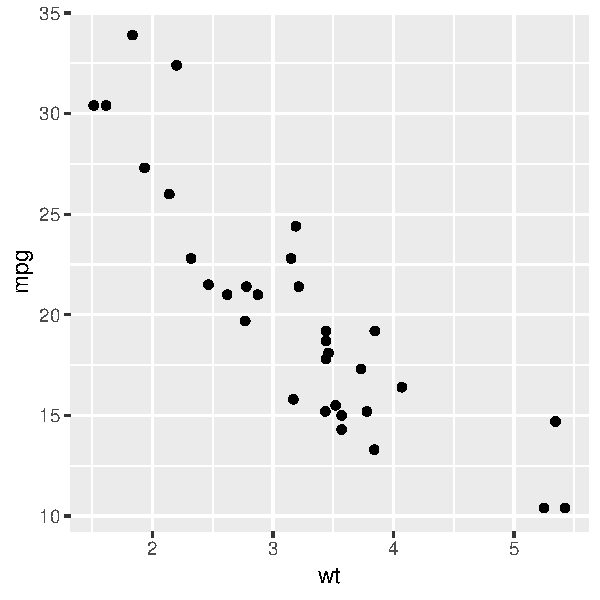
\includegraphics[width=0.5\linewidth]{ggplots2loon_files/figure-latex/mpg vs wt ggplot display-1} \end{center}

We might also display a histogram of some other variate, say the
engine's horsepower \texttt{hp}. In \texttt{ggplot2} this would be
constructed as

\begin{Shaded}
\begin{Highlighting}[]
\NormalTok{h1 <-}\StringTok{ }\KeywordTok{ggplot}\NormalTok{(mtcars, }\KeywordTok{aes}\NormalTok{(hp)) }\OperatorTok{+}\StringTok{ }\KeywordTok{geom_histogram}\NormalTok{()}
\end{Highlighting}
\end{Shaded}

and displayed as

\begin{Shaded}
\begin{Highlighting}[]
\NormalTok{h1}
\end{Highlighting}
\end{Shaded}

\begin{center}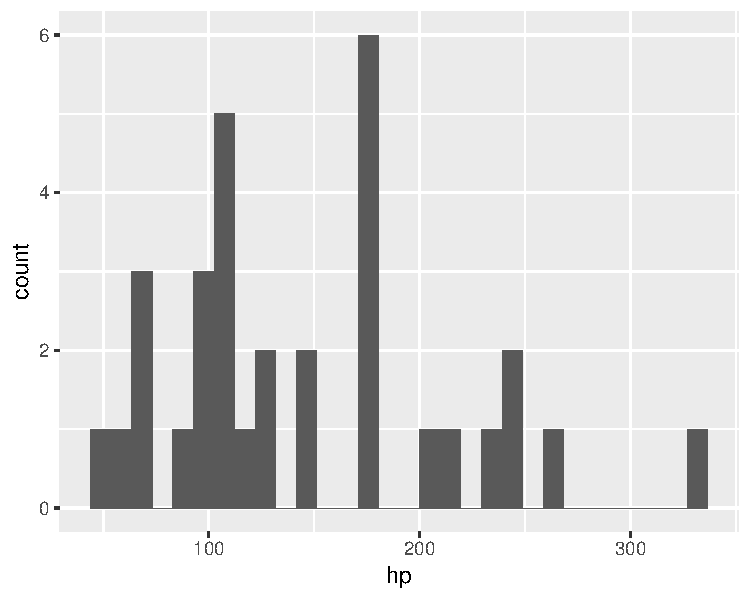
\includegraphics[width=0.5\linewidth]{ggplots2loon_files/figure-latex/hp ggplot display-1} \end{center}

\subsection{loon.ggplot() and
grid.loon()}\label{loon.ggplot-and-grid.loon}

Using the \texttt{loon.ggplot} package, the \texttt{"ggplot"} data
structures \texttt{p1} and \texttt{h1} can be \textbf{turned into an
interactive loon plot} using the \texttt{loon.ggplot()} function:

\begin{Shaded}
\begin{Highlighting}[]
\KeywordTok{library}\NormalTok{(loon.ggplot)}
\NormalTok{l_p1 <-}\StringTok{ }\KeywordTok{loon.ggplot}\NormalTok{(p1)  }\CommentTok{# the scatterplot}
\NormalTok{l_h1 <-}\StringTok{ }\KeywordTok{loon.ggplot}\NormalTok{(h1)  }\CommentTok{# the histogram}
\end{Highlighting}
\end{Shaded}

These loon plots should look very much (though not exactly) like the
ggplot from which it was constructed. Using \texttt{grid.loon()}
\texttt{grid} graphics versions of the loon plots can be created for
static display, printing, and incorporation into documents:

\begin{Shaded}
\begin{Highlighting}[]
\KeywordTok{grid.loon}\NormalTok{(l_p1)}
\end{Highlighting}
\end{Shaded}

\begin{center}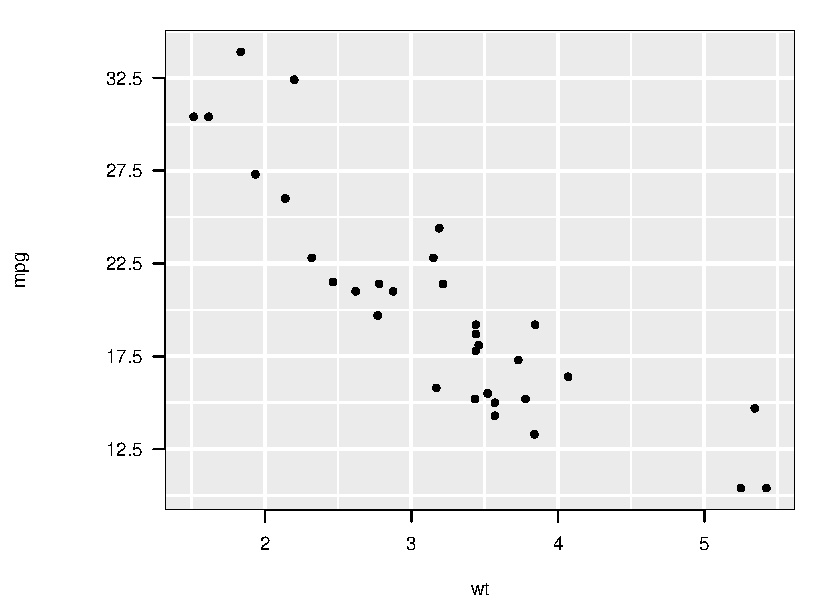
\includegraphics[width=0.5\linewidth]{ggplots2loon_files/figure-latex/grid version of l_p1-1} \end{center}

\begin{Shaded}
\begin{Highlighting}[]
\KeywordTok{grid.loon}\NormalTok{(l_h1)}
\end{Highlighting}
\end{Shaded}

\begin{center}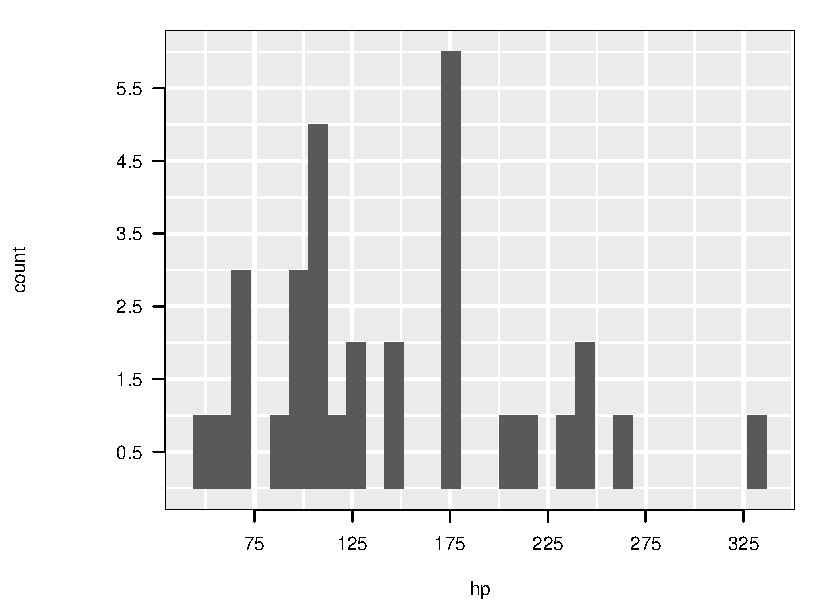
\includegraphics[width=0.5\linewidth]{ggplots2loon_files/figure-latex/grid version of l_h1-1} \end{center}

\subsection{interaction - direct
manipulation}\label{interaction---direct-manipulation}

Unlike \texttt{p1} and \texttt{h1}, the loon counterparts \texttt{l\_p1}
and \texttt{l\_h1} are both \textbf{interactive}; their displays can be
changed by \textbf{direct manipulation} using the mouse and/or each loon
plot's \textbf{loon inspector}.

\begin{center}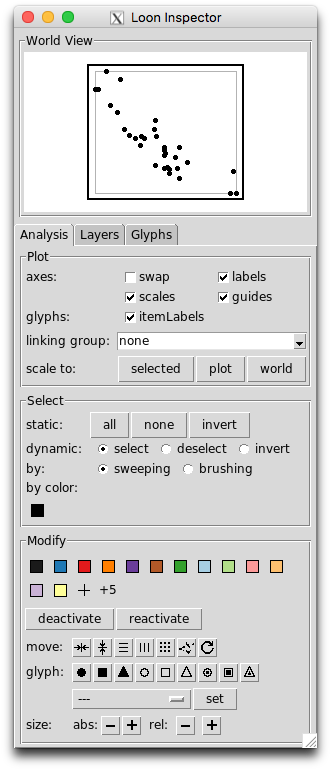
\includegraphics[width=0.25\linewidth]{./img/ggplots2loon//inspector_l_p1} \end{center}

For example, points in the loon scatterplot \texttt{l\_p1}, can be
selected with a mouse (\texttt{\textless{}SHIFT\textgreater{}} select
for multiple selection) and their glyph changed in shape or color, for
example. Scrolling over the plot causes zooming and
\texttt{\textless{}RIGHT-BUTTON\textgreater{}} (or
\texttt{\textless{}SECONDARY-BUTTON\textgreater{}}, depending on your
mouse setup) can be used to pan the plot (the same can be done via the
``World View'' of the inspector).

If, for example, the \texttt{itemLabels} box is checked in the
inspector, then hovering over any point will pop a little ``tool tip''
identifying the point.

Similarly, the loon histogram \texttt{l\_h1} has many interactions and a
specialized loon inspector. For example, the histogram can be changed
from \texttt{frequency} to \texttt{density} in the inspector and the
``bin handle'' turned on and off; the latter can be directly manipulated
to change the size and location of the bins whenever it appears on the
histogram plot.

Many, many, more interactions are possible. You might want to experiment
with the plot and the inspector to see some of the possibilities.
(\textbf{Recommended:} explore the vignettes given in the \texttt{loon}
package).

\subsubsection{linking}\label{linking}

One of the basic features of interactive statistical graphics is the
ability to \textbf{link displays}. In loon this is most easily
accomplished via the loon inspector.

To see the effect, with the mouse select one of the loon plots
\texttt{l\_p1} or \texttt{l\_h1} and then select the inspector. On the
inspector, type the text \texttt{mtcars} into the text input box which
appears next to ``linking group''; then hit return/enter. As a result,
the text appearing there will be \texttt{mtcars\ {[}1\ linked{]}}; this
shows that the selected plot is participating in the linking group named
``mtcars'' and that it is presently the only one so linked.

Now select the other plot \texttt{l\_h1} or \texttt{l\_p1}. On the loon
inspector for this plot, you can again enter ``mtcars'' as this plot's
linking group (this can be done as before or selected from the menu
accessible from the down arrow next to the linking group. As soon as the
second plot is linked, the user is prompted to choose how to synchronize
the linked features of the new plot to the previous plot. The choice is
between \emph{pushing} the display features from the current plot to the
rest of the plots in the group and \emph{pulling} the display features
from the group to change those of the current plot. The resulting
linking group entry should now show \texttt{mtcars\ {[}2\ linked{]}}.

Once the both plots are in the same linking group (i.e. ``mtcars''),
selections in one plot will be reflected in the other. Try this. To see
colour changes in the histogram, the box \texttt{stacked\ colors} must
be checked.

Linking is one way to condition on the values in one plot and observe
their effect in the others. Try this with ``brushing'' in either plot.

\subsection{interaction -
programmatic}\label{interaction---programmatic}

The loon plot, \texttt{l\_p1} is itself a data structure of class
\texttt{"l\_plot"} and \texttt{"loon"}

\begin{Shaded}
\begin{Highlighting}[]
\KeywordTok{class}\NormalTok{(l_p1)}
\CommentTok{#> [1] "l_plot" "loon"}
\NormalTok{l_p1}
\CommentTok{#> [1] ".1.plot"}
\CommentTok{#> attr(,"class")}
\CommentTok{#> [1] "l_plot" "loon"}
\end{Highlighting}
\end{Shaded}

whose value is a string which uniquely identifies it. As such, it can be
interacted with programmatically as well as by direct manipulation using
the mouse and/or the plot's loon inspector.

For example, via direct manipulation, the plot might have zoomed or
panned so that many of the points no longer appear in the plot. The plot
can be returned to its original position and scaling (either through the
loon inspector's \texttt{scale\ to:\ plot} or) by calling the function
\texttt{l\_scaleto\_plot()} programmatically on the loon data structure
\texttt{l\_p1} as in

\begin{Shaded}
\begin{Highlighting}[]
\KeywordTok{l_scaleto_plot}\NormalTok{(l_p1)}
\end{Highlighting}
\end{Shaded}

As a base loon structure, an \texttt{l\_plot} has a variety of
\texttt{l\_info\_states} available that can be accessed and/or set. The
names of these states are had with
\texttt{names(l\_info\_states(l\_p1))} or more simply with

\begin{Shaded}
\begin{Highlighting}[]
\KeywordTok{names}\NormalTok{(l_p1)}
\CommentTok{#>  [1] "glyph"            "itemLabel"        "showItemLabels"  }
\CommentTok{#>  [4] "linkingGroup"     "linkingKey"       "zoomX"           }
\CommentTok{#>  [7] "zoomY"            "panX"             "panY"            }
\CommentTok{#> [10] "deltaX"           "deltaY"           "xlabel"          }
\CommentTok{#> [13] "ylabel"           "title"            "showLabels"      }
\CommentTok{#> [16] "showScales"       "swapAxes"         "showGuides"      }
\CommentTok{#> [19] "background"       "foreground"       "guidesBackground"}
\CommentTok{#> [22] "guidelines"       "minimumMargins"   "labelMargins"    }
\CommentTok{#> [25] "scalesMargins"    "x"                "y"               }
\CommentTok{#> [28] "xTemp"            "yTemp"            "color"           }
\CommentTok{#> [31] "selected"         "active"           "size"            }
\CommentTok{#> [34] "tag"              "useLoonInspector" "selectBy"        }
\CommentTok{#> [37] "selectionLogic"}
\end{Highlighting}
\end{Shaded}

Their values can be accessed using the \texttt{{[}{]}} function. For
example, the background grid lines which appear by default on ggplots,
are called ``guides'' in loon and the logical state determining whether
they appear or not in the loon plot is \texttt{"showGuides"}, accessed
as

\begin{Shaded}
\begin{Highlighting}[]
\NormalTok{l_p1[}\StringTok{"showGuides"}\NormalTok{]}
\CommentTok{#> [1] TRUE}
\end{Highlighting}
\end{Shaded}

These can be turned off (loon default) or on (ggplot default) by simply
changing this value -- either through the \texttt{guides} check box in
the inspector or programmatically as

\begin{Shaded}
\begin{Highlighting}[]
\CommentTok{# Turn the guides off}
\NormalTok{l_p1[}\StringTok{"showGuides"}\NormalTok{] <-}\StringTok{ }\OtherTok{FALSE}
\CommentTok{# Turn the guides on again}
\NormalTok{l_p1[}\StringTok{"showGuides"}\NormalTok{] <-}\StringTok{ }\OtherTok{TRUE}
\end{Highlighting}
\end{Shaded}

All other info states can also be changed programmatically as well. For
example, a title could be added, the axis labels changed, and a highly
informative \texttt{"itemLabel"} given for each car.

\begin{Shaded}
\begin{Highlighting}[]
\NormalTok{l_p1[}\StringTok{"title"}\NormalTok{] <-}\StringTok{ "1974 Motor Trend Car Road Tests"}
\NormalTok{l_p1[}\StringTok{"xlabel"}\NormalTok{] <-}\StringTok{ "Curb weight (1000s of lbs)"}
\NormalTok{l_p1[}\StringTok{"ylabel"}\NormalTok{] <-}\StringTok{ "Gas mileage (miles per US gallon)"}
\NormalTok{newlabels <-}\StringTok{ }\KeywordTok{paste0}\NormalTok{(}\KeywordTok{rownames}\NormalTok{(mtcars), }\StringTok{"}\CharTok{\textbackslash{}n}\StringTok{   "}\NormalTok{,}
                    \KeywordTok{c}\NormalTok{(}\StringTok{"V-"}\NormalTok{, }\StringTok{"straight-"}\NormalTok{)[mtcars}\OperatorTok{$}\NormalTok{vs }\OperatorTok{+}\StringTok{ }\DecValTok{1}\NormalTok{], mtcars}\OperatorTok{$}\NormalTok{cyl, }\StringTok{" }\CharTok{\textbackslash{}n}\StringTok{   "}\NormalTok{, }
\NormalTok{                    mtcars}\OperatorTok{$}\NormalTok{disp, }\StringTok{" cubic inch }\CharTok{\textbackslash{}n}\StringTok{   "}\NormalTok{, }
\NormalTok{                    mtcars}\OperatorTok{$}\NormalTok{gear, }\StringTok{" speed }\CharTok{\textbackslash{}n}\StringTok{   "}\NormalTok{, }
                    \KeywordTok{c}\NormalTok{(}\StringTok{"automatic"}\NormalTok{, }\StringTok{"manual"}\NormalTok{)[mtcars}\OperatorTok{$}\NormalTok{am }\OperatorTok{+}\StringTok{ }\DecValTok{1}\NormalTok{]}
\NormalTok{                    )}
\NormalTok{l_p1[}\StringTok{"itemLabel"}\NormalTok{] <-}\StringTok{ }\NormalTok{newlabels}
\NormalTok{l_p1[}\StringTok{"showItemLabels"}\NormalTok{] <-}\StringTok{ }\OtherTok{TRUE}
\end{Highlighting}
\end{Shaded}

The last line above ensures its item label appears whenever the mouse
hovers over any point. This gives some interesting information to the
curious autophile.

The points might also be visibly distinguished by the transmission type
and the number of cylinders of its engine. Glyph type could distinguish
transmissions and colour the number of cylinders. (To better distinguish
shapes, we also make the glyphs fairly large via the \texttt{size}
state.)

\begin{Shaded}
\begin{Highlighting}[]
\NormalTok{l_p1[}\StringTok{"size"}\NormalTok{] <-}\StringTok{ }\DecValTok{10}
\NormalTok{l_p1[}\StringTok{"glyph"}\NormalTok{][mtcars}\OperatorTok{$}\NormalTok{am }\OperatorTok{==}\StringTok{ }\DecValTok{0}\NormalTok{] <-}\StringTok{ "ccircle"}
\NormalTok{l_p1[}\StringTok{"glyph"}\NormalTok{][mtcars}\OperatorTok{$}\NormalTok{am }\OperatorTok{==}\StringTok{ }\DecValTok{1}\NormalTok{] <-}\StringTok{ "triangle"}
\NormalTok{gears <-}\StringTok{ }\KeywordTok{sort}\NormalTok{(}\KeywordTok{unique}\NormalTok{(mtcars}\OperatorTok{$}\NormalTok{gear))}
\NormalTok{ngears <-}\StringTok{ }\KeywordTok{length}\NormalTok{(gears)}
\NormalTok{cols <-}\StringTok{ }\KeywordTok{c}\NormalTok{(}\StringTok{"lightblue"}\NormalTok{, }\StringTok{"steelblue"}\NormalTok{, }\StringTok{"black"}\NormalTok{)}
\ControlFlowTok{for}\NormalTok{ (i }\ControlFlowTok{in} \DecValTok{1}\OperatorTok{:}\NormalTok{ngears) \{}
\NormalTok{  l_p1[}\StringTok{"color"}\NormalTok{][mtcars}\OperatorTok{$}\NormalTok{gear }\OperatorTok{==}\StringTok{ }\NormalTok{gears[i]] <-}\StringTok{ }\NormalTok{cols[i]}
\NormalTok{\}}
\end{Highlighting}
\end{Shaded}

We might then zoom in on the \texttt{"black"} coloured points (note that
these are now \texttt{hex\ colors}), and maybe remove the others from
the display (temporarily render them inactive) as follows.

\begin{Shaded}
\begin{Highlighting}[]
\NormalTok{l_p1[}\StringTok{"active"}\NormalTok{] <-}\StringTok{ }\NormalTok{l_p1[}\StringTok{"color"}\NormalTok{] }\OperatorTok{==}\StringTok{ }\KeywordTok{l_hexcolor}\NormalTok{(}\StringTok{"black"}\NormalTok{)}
\KeywordTok{l_scaleto_active}\NormalTok{(l_p1)}
\NormalTok{l_p1[}\StringTok{"title"}\NormalTok{] <-}\StringTok{ "5 speed manual transmission"}
\end{Highlighting}
\end{Shaded}

The plot should now look something like this (a \texttt{grid} graphics
version of \texttt{l\_p1}):

\begin{Shaded}
\begin{Highlighting}[]
\KeywordTok{grid.loon}\NormalTok{(l_p1)}
\end{Highlighting}
\end{Shaded}

\begin{center}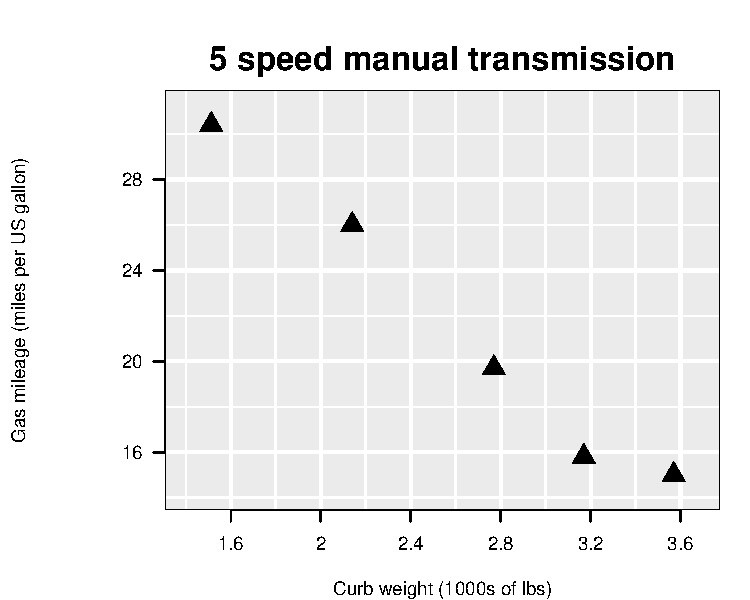
\includegraphics[width=0.7\linewidth]{ggplots2loon_files/figure-latex/high gear manual grid plot-1} \end{center}

Again, the plot can be returned to its original scale with all points
reactivated as follows:

\begin{Shaded}
\begin{Highlighting}[]
\NormalTok{l_p1[}\StringTok{"active"}\NormalTok{] <-}\StringTok{ }\OtherTok{TRUE}
\KeywordTok{l_scaleto_plot}\NormalTok{(l_p1)}
\NormalTok{l_p1[}\StringTok{"title"}\NormalTok{] <-}\StringTok{ "All points again"}
\KeywordTok{grid.loon}\NormalTok{(l_p1)}
\end{Highlighting}
\end{Shaded}

\begin{center}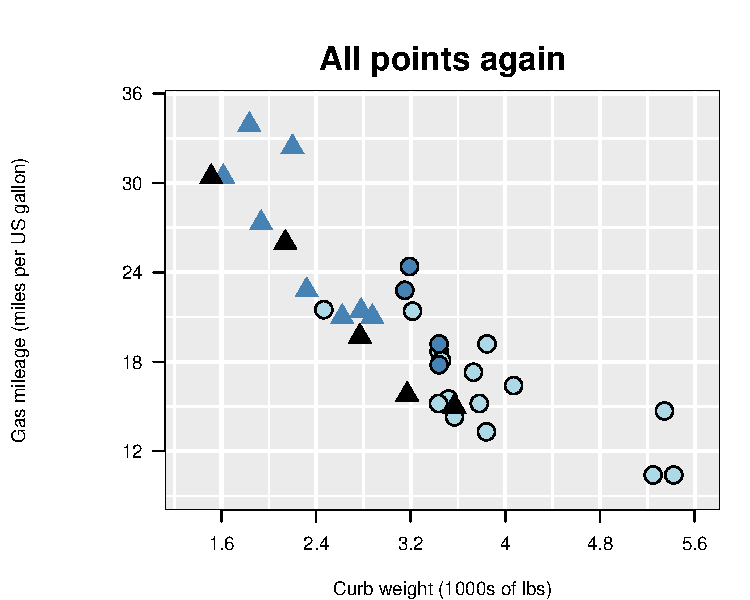
\includegraphics[width=0.7\linewidth]{ggplots2loon_files/figure-latex/Back to all points-1} \end{center}

\subsubsection{linking}\label{linking-1}

In loon, plots are linked only if they are in the same
\texttt{linkingGroup} (which can be any string that meaningfully
identifies the group of plots). The \texttt{linkingGroup} can also be
set programmatically. For the \textbf{first} plot in a linking group,
this can be set using the square bracket notation as above. For example,
instead of ``mtcars'' we might want a more meaningful string for the
linking group for \texttt{l\_p1}.

\begin{Shaded}
\begin{Highlighting}[]
\NormalTok{l_p1[}\StringTok{"linkingGroup"}\NormalTok{] <-}\StringTok{ "Motor Trend 1974"}
\end{Highlighting}
\end{Shaded}

The two plots \texttt{l\_p1} and \texttt{l\_h1} are now no longer linked
because they are no longer in the same linking group.

To add \texttt{l\_h1} to this new linking group called ``Motor Trend
1974'', \textbf{the square bracket assignment will no longer work}. This
is because the two plots must be synchronized at the time any plot is
added to an existing group. Instead, \texttt{l\_h1} (and any subsequent
plot) must be added to the group using the \texttt{l\_configure()}
function as follows:

\begin{Shaded}
\begin{Highlighting}[]
\KeywordTok{l_configure}\NormalTok{(l_h1, }\DataTypeTok{linkingGroup =} \StringTok{"Motor Trend 1974"}\NormalTok{, }\DataTypeTok{sync =} \StringTok{"pull"}\NormalTok{)}
\end{Highlighting}
\end{Shaded}

Notice, by the way, that the (stacked) colours in the histogram will
follow those of \texttt{l\_p1}. For example,

\begin{Shaded}
\begin{Highlighting}[]
\NormalTok{l_h1[}\StringTok{"showStackedColors"}\NormalTok{] <-}\StringTok{ }\OtherTok{TRUE}
\KeywordTok{grid.loon}\NormalTok{(l_h1)}
\end{Highlighting}
\end{Shaded}

\begin{center}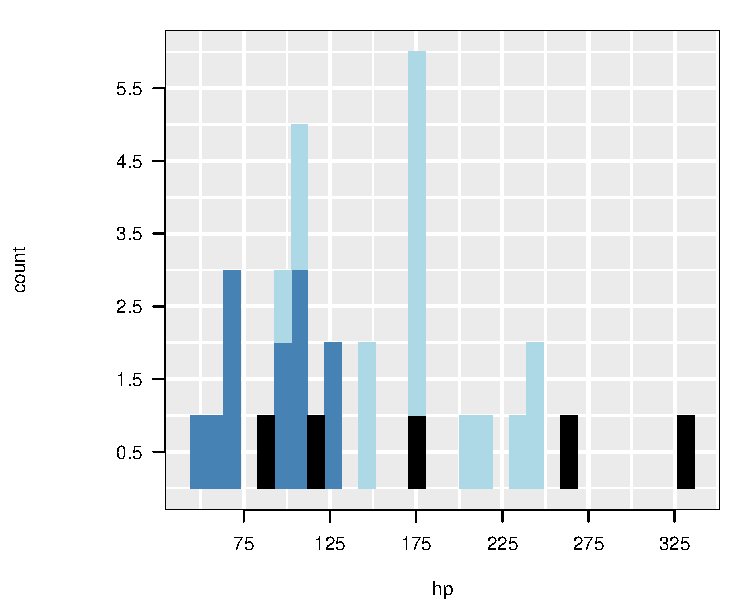
\includegraphics[width=0.7\linewidth]{ggplots2loon_files/figure-latex/stacked colours grid.loon-1} \end{center}

\subsubsection{linking with
loon.ggplot()}\label{linking-with-loon.ggplot}

It is possible to declare the linking group of the loon plot at the time
it is created from the ggplot.

For example, the relationship between the acceleration and the drive
axle ratio could be of interest; these are measured by the time taken to
accelerate to a quarter mile, \texttt{qsec}, and \texttt{drat}. The
\texttt{gplot} is

\begin{Shaded}
\begin{Highlighting}[]
\CommentTok{# First using another ggplot}
\NormalTok{p2 <-}\StringTok{ }\KeywordTok{ggplot}\NormalTok{(mtcars, }\KeywordTok{aes}\NormalTok{(}\DataTypeTok{x =}\NormalTok{ drat, }\DataTypeTok{y =}\NormalTok{ qsec)) }\OperatorTok{+}\StringTok{ }\KeywordTok{geom_point}\NormalTok{()}
\end{Highlighting}
\end{Shaded}

which looks like

\begin{Shaded}
\begin{Highlighting}[]
\NormalTok{p2}
\end{Highlighting}
\end{Shaded}

\begin{center}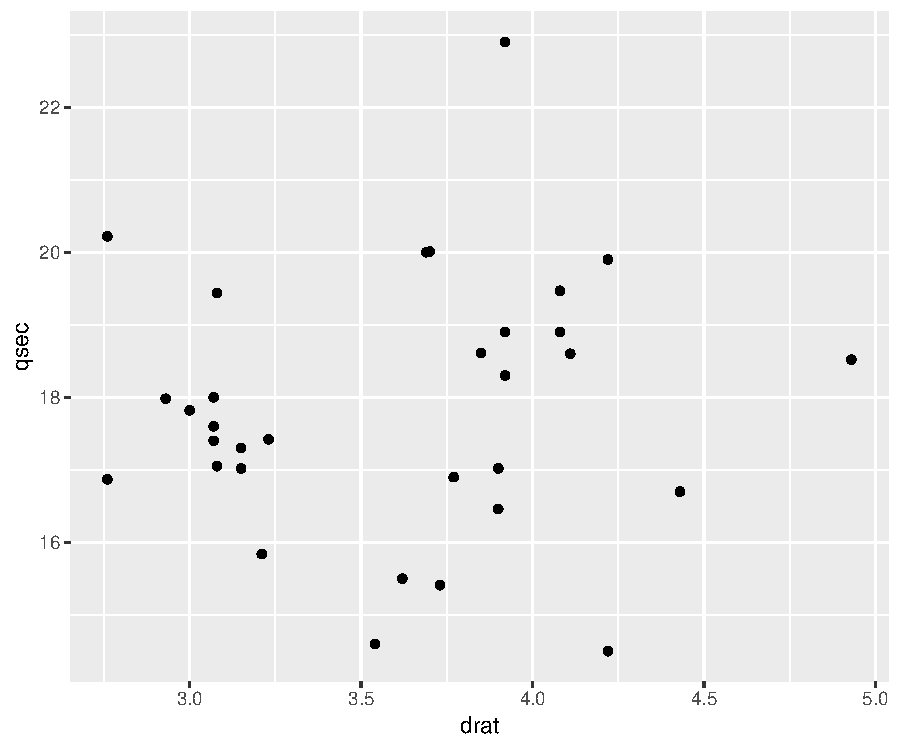
\includegraphics[width=0.5\linewidth]{ggplots2loon_files/figure-latex/ggplot p2-1} \end{center}

The corresponding loon plot can be linked immediately when it is created

\begin{Shaded}
\begin{Highlighting}[]
\NormalTok{l_p2 <-}\StringTok{ }\KeywordTok{loon.ggplot}\NormalTok{(p2, }
                    \DataTypeTok{linkingGroup =} \StringTok{"Motor Trend 1974"}\NormalTok{,}
                    \DataTypeTok{title =} \StringTok{"Acceleration measures"}\NormalTok{, }
                    \DataTypeTok{xlabel =} \StringTok{"Drive axle ratio"}\NormalTok{,}
                    \DataTypeTok{ylabel =} \StringTok{"Quarter mile (seconds)"}\NormalTok{,}
                    \DataTypeTok{itemLabel =}\NormalTok{ newlabels)}
\end{Highlighting}
\end{Shaded}

as can any other state of a loon plot, such as \texttt{title},
\texttt{xlabel}, \texttt{ylabel,\ or}itemLabel` as shown here.

The points in the loon plot inherit their colours from the linking group
``Motor Trend 1974'':

\begin{Shaded}
\begin{Highlighting}[]
\KeywordTok{grid.loon}\NormalTok{(l_p2)}
\end{Highlighting}
\end{Shaded}

\begin{center}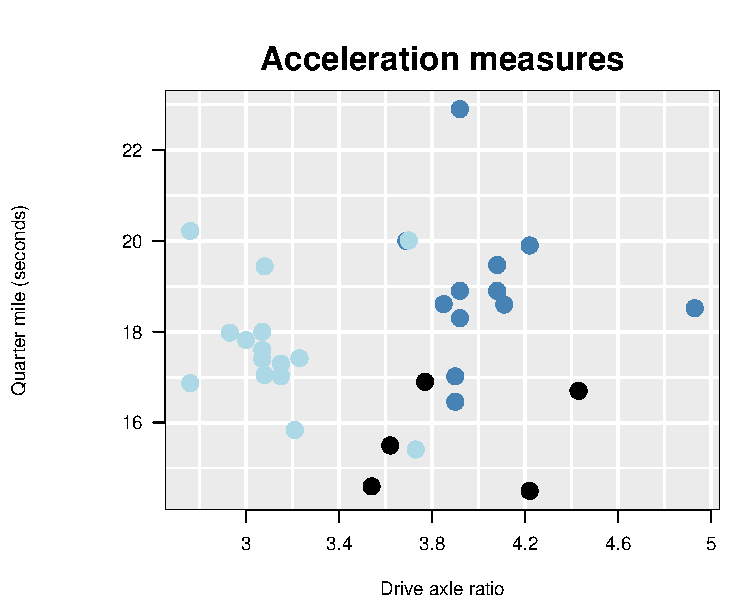
\includegraphics[width=0.7\linewidth]{ggplots2loon_files/figure-latex/loon plot l_p2-1} \end{center}

Note that \texttt{l\_p2} did not inherit the shapes of its points from
the \texttt{l\_p1}. That is because only those states that have been
defined as \texttt{linkedStates} are shared by any given plot.

\subsubsection{linked states}\label{linked-states}

The \texttt{linkedStates} of any plot are those which that plot will
share (and hence update) with any other plot in the same
\texttt{linkingGroup}. The default states that are linked for an
\texttt{l\_plot} like \texttt{l\_p1} are

\begin{Shaded}
\begin{Highlighting}[]
\KeywordTok{l_getLinkedStates}\NormalTok{(l_p1)}
\CommentTok{#> [1] "color"    "selected" "active"   "size"}
\end{Highlighting}
\end{Shaded}

and a change in any of these states by any plot in the linking group
will cause the same change in these states on \texttt{l\_p1}. These are
the same states linked by \texttt{l\_p2}.

In contrast, the loon histogram \texttt{l\_h1} has default linked states

\begin{Shaded}
\begin{Highlighting}[]
\KeywordTok{l_getLinkedStates}\NormalTok{(l_h1)}
\CommentTok{#> [1] "color"    "selected" "active"}
\end{Highlighting}
\end{Shaded}

which excludes \texttt{size} as not a meaningful state for a loon
histogram (class \texttt{l\_hist}).

The linked states can be modified. For example, we might choose to not
have the second plot respond to changes in the ``active'' state of other
plots in the same linking group. This is effected by reducing the states
for just the plot \texttt{l\_p2}

\begin{Shaded}
\begin{Highlighting}[]
\KeywordTok{l_setLinkedStates}\NormalTok{(l_p1,  }\KeywordTok{c}\NormalTok{(}\StringTok{"color"}\NormalTok{, }\StringTok{"selected"}\NormalTok{, }\StringTok{"size"}\NormalTok{))}
\end{Highlighting}
\end{Shaded}

A more sophisticated change would be also link the glyphs used for each
point between plots. This will \emph{typically} be the shape of the
glyph. (\textbf{Warning}: but not always. For example, when images are
used for the points, a little more care needs to be taken). To do this
for both \texttt{l\_p1} and \texttt{l\_p2} we add to the states being
linked as follows.

\begin{Shaded}
\begin{Highlighting}[]
\KeywordTok{l_setLinkedStates}\NormalTok{(l_p1, }\KeywordTok{c}\NormalTok{(}\StringTok{"glyph"}\NormalTok{, }\KeywordTok{l_getLinkedStates}\NormalTok{(l_p1)))}
\KeywordTok{l_setLinkedStates}\NormalTok{(l_p2, }\KeywordTok{c}\NormalTok{(}\StringTok{"glyph"}\NormalTok{, }\KeywordTok{l_getLinkedStates}\NormalTok{(l_p2)))}
\end{Highlighting}
\end{Shaded}

Now any \textbf{change} to the glyphs in either plot will change the
glyphs in both.

\begin{Shaded}
\begin{Highlighting}[]
\NormalTok{triangles <-}\StringTok{ }\NormalTok{l_p1[}\StringTok{"glyph"}\NormalTok{] }\OperatorTok{==}\StringTok{ "triangle"}
\NormalTok{l_p1[}\StringTok{"glyph"}\NormalTok{][triangles] <-}\StringTok{ "ctriangle"}
\end{Highlighting}
\end{Shaded}

Here now for \texttt{l\_p1}

\begin{Shaded}
\begin{Highlighting}[]
\KeywordTok{grid.loon}\NormalTok{(l_p1)}
\end{Highlighting}
\end{Shaded}

\begin{center}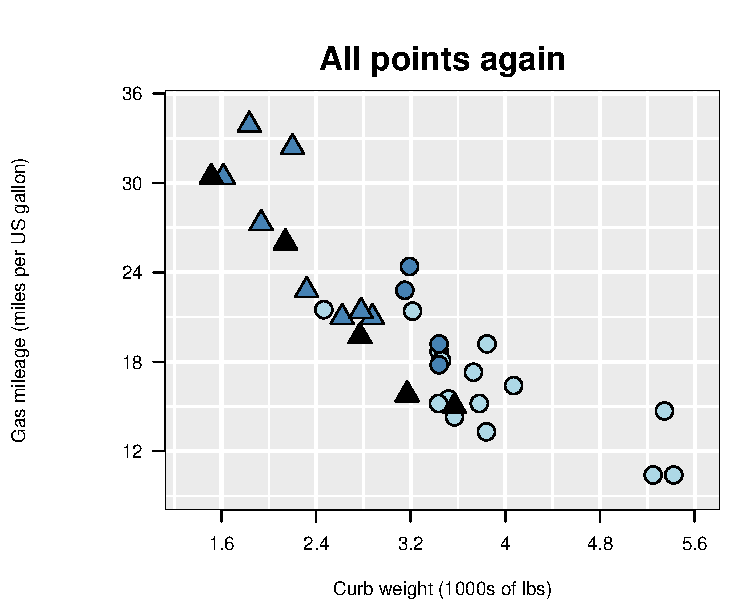
\includegraphics[width=0.7\linewidth]{ggplots2loon_files/figure-latex/changed glyphs l_p1-1} \end{center}

and propagated to \texttt{l\_p2}

\begin{Shaded}
\begin{Highlighting}[]
\KeywordTok{grid.loon}\NormalTok{(l_p2)}
\end{Highlighting}
\end{Shaded}

\begin{center}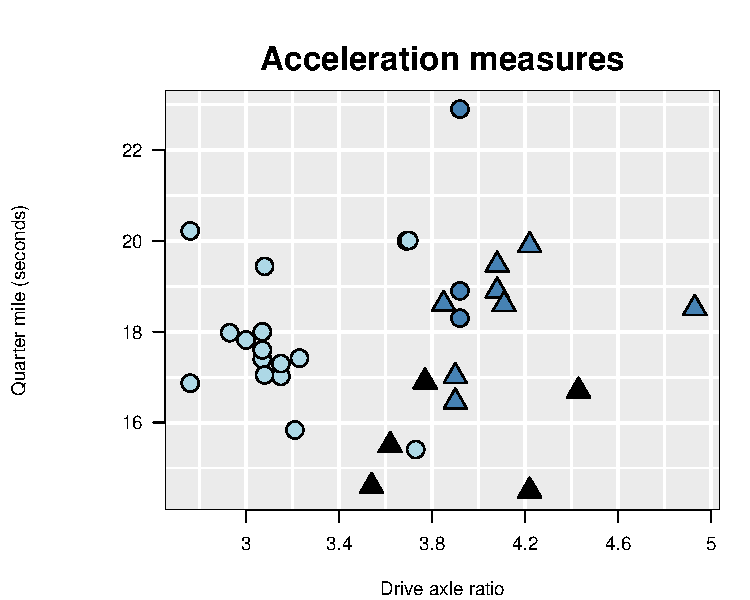
\includegraphics[width=0.7\linewidth]{ggplots2loon_files/figure-latex/changed glyphs l_p2-1} \end{center}

\section{Layers}\label{layers}

Rather complex plots can be built up in \texttt{ggplot2} by adding
\emph{layers}. For example,

\begin{Shaded}
\begin{Highlighting}[]
\NormalTok{p_fit <-}\StringTok{ }\KeywordTok{ggplot}\NormalTok{(mtcars, }\KeywordTok{aes}\NormalTok{(drat, mpg)) }\OperatorTok{+}\StringTok{ }\KeywordTok{geom_smooth}\NormalTok{() }\OperatorTok{+}\StringTok{ }\KeywordTok{geom_point}\NormalTok{()}
\NormalTok{p_fit}
\end{Highlighting}
\end{Shaded}

\begin{center}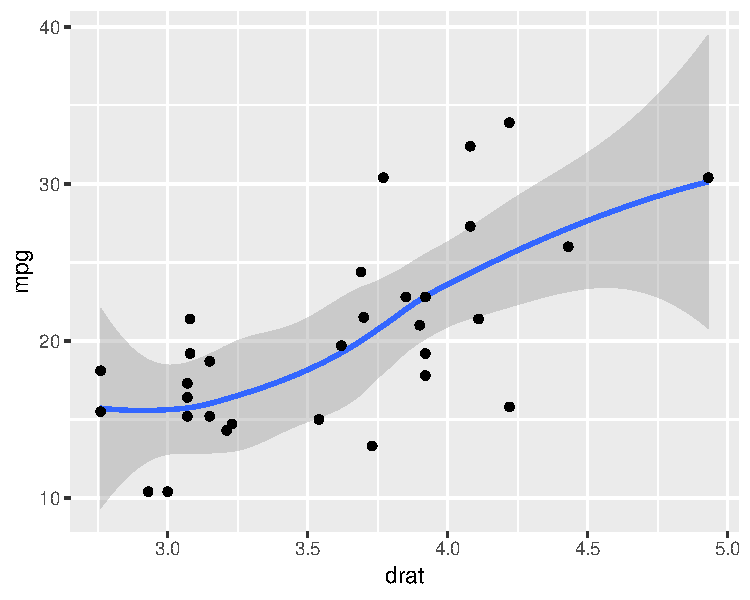
\includegraphics[width=0.7\linewidth]{ggplots2loon_files/figure-latex/mtcars smooth-1} \end{center}

The \textbf{corresponding interactive} loon plot is

\begin{Shaded}
\begin{Highlighting}[]
\NormalTok{l_p_fit <-}\StringTok{ }\KeywordTok{loon.ggplot}\NormalTok{(p_fit)}
\end{Highlighting}
\end{Shaded}

As with ggplots (and grid graphics plots), loon plots have layers. These
can be identified (and manipulated) by selecting the ``Layers'' tab of
the inspector.

\begin{center}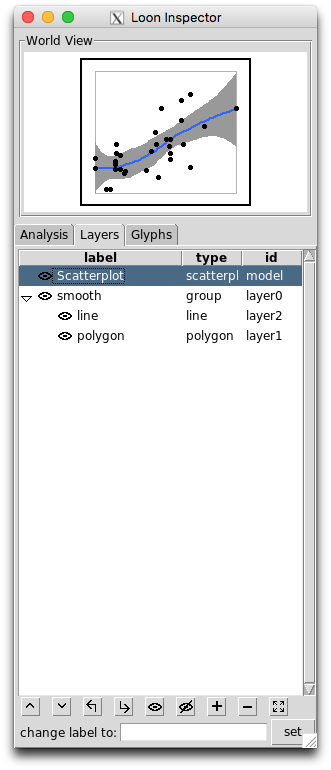
\includegraphics[width=0.25\linewidth]{./img/ggplots2loon//inspector_l_p_fit} \end{center}

As can be seen, four distinct layers appear. There is the scatterplot
(from \texttt{geom\_point()}), then a group layer called the
\texttt{smooth} which has been opened up here by toggling the triangle
at its left to reveal it is composed of a \texttt{line} and a
\texttt{polygon} layer (in that order).

The \textbf{order of the layers is important} and represent their visual
order in the corresponding plot. By default, these will follow the order
in which the various \texttt{geom}s appear in the construction of the
ggplot. For example, had \texttt{geom\_point()} appeared before the
\texttt{geom\_smooth()} in the left to right reading of the ggplot
construction, then the \texttt{Scatterplot} layer would have appeared
below the \texttt{smooth} group layer and visually obscured all points
at the same location.

\begin{center}
*In loon, layer order is display order.*
\end{center}

The order of display can be changed from the inspector via the first two
buttons at the bottom left of the layers panel. The order can also be
changed programmatically. For example, the scatterplot can be moved
lower in the display order as

\begin{Shaded}
\begin{Highlighting}[]
\KeywordTok{l_layer_lower}\NormalTok{(l_p_fit, }\StringTok{"model"}\NormalTok{)}
\end{Highlighting}
\end{Shaded}

and raised back up again so that the points are again on top

\begin{Shaded}
\begin{Highlighting}[]
\KeywordTok{l_layer_raise}\NormalTok{(l_p_fit, }\StringTok{"model"}\NormalTok{)}
\end{Highlighting}
\end{Shaded}

Note that the scatterplot layer identified by its ``layer id'', namely
the string \texttt{"model"}. The function
\texttt{l\_layer\_ids(\ l\_p\_fit\ )} will return a list of all the
layer ids from its argument \texttt{l\_p\_fit}.

Reading left to right, the remaining buttons on the bottom of the layers
tab on the inspector allow a (selected) layer to be moved out of a
group, into a group, made visible, or made invisible, and add a new
group layer, delete any layer, or scale the plot to the selected layer.
All of these can also be achieved programmatically and numerous other
functions exist in loon to add new layers -- see
\texttt{help("l\_layer")} or \texttt{l\_help("learn\_R\_layer")} for the
range of possibilities.

\subsection{the model layer}\label{the-model-layer}

There is always one layer in loon that is the \textbf{active layer}
which at present is always identified as the ``model'' layer. It is this
layer which fields mouse events such as selection and brushing; it is
also the layer that reacts to changes in linking states.

In loon, scatterplots and histograms can be identified as the ``model''
layer (the former produced via the \texttt{l\_plot()} function, the
latter via \texttt{l\_hist()}).

A loon \texttt{l\_plot()} corresponds to a ggplot \texttt{geom\_point()}
and a loon \texttt{l\_hist()} to a ggplot \texttt{geom\_histogram()}.\\
In \texttt{ggplot2} several \texttt{geom}s might appear in the
construction of a plot, each one providing a layer. But in \texttt{loon}
only one layer, namely the \texttt{"model"} layer, can be active. This
means which of the ggplot layers are intended to be the active
\texttt{"model"} layer in loon must be determined at the time of
construction (the call to \texttt{loon.ggplot()}).

Consider the following example where three \texttt{geom}s are created as
layers in the ggplot. Here a histogram (on a density scale) is overlaid
with a scatter of points along the horizontal axis, and then with a
curve from a density estimate.

\begin{Shaded}
\begin{Highlighting}[]
\NormalTok{p_hdp <-}\StringTok{ }\KeywordTok{ggplot}\NormalTok{(mtcars, }\KeywordTok{aes}\NormalTok{(}\DataTypeTok{x =}\NormalTok{ wt, }\DataTypeTok{y =}\NormalTok{ ..density..)) }\OperatorTok{+}
\StringTok{  }\KeywordTok{geom_histogram}\NormalTok{(}\DataTypeTok{binwidth =} \FloatTok{0.5}\NormalTok{, }
                 \DataTypeTok{fill =} \StringTok{"grey"}\NormalTok{, }
                 \DataTypeTok{color =} \StringTok{"red"}\NormalTok{) }\OperatorTok{+}
\StringTok{  }\KeywordTok{geom_density}\NormalTok{(}\DataTypeTok{color =} \StringTok{"firebrick"}\NormalTok{, }\DataTypeTok{lwd =} \FloatTok{1.5}\NormalTok{) }\OperatorTok{+}
\StringTok{  }\KeywordTok{geom_point}\NormalTok{(}\DataTypeTok{data =} \KeywordTok{data.frame}\NormalTok{(}\DataTypeTok{x =}\NormalTok{ mtcars}\OperatorTok{$}\NormalTok{wt, }\DataTypeTok{y =} \DecValTok{0}\NormalTok{), }
             \DataTypeTok{mapping =} \KeywordTok{aes}\NormalTok{(x, y), }
             \DataTypeTok{color =} \StringTok{"firebrick"}\NormalTok{, }\DataTypeTok{size =} \DecValTok{3}\NormalTok{)}
\CommentTok{# the ggplot}
\NormalTok{p_hdp}
\end{Highlighting}
\end{Shaded}

\begin{center}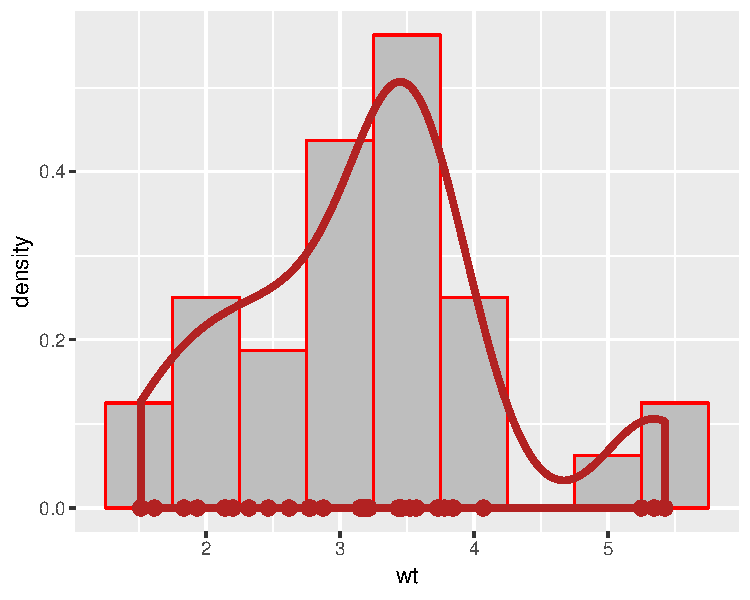
\includegraphics[width=0.7\linewidth]{ggplots2loon_files/figure-latex/multiple geoms-1} \end{center}

To render this in loon, which layer will be interactive needs to be
determined. By default, this will be the first layer appearing in the
construction of the ggplot -- in this case the the histogram. The
scatter of points will not be interactive and there are presently no
interactive curves in a loon plot.

\subsubsection{\texorpdfstring{specifying the active \texttt{geom}
layer}{specifying the active geom layer}}\label{specifying-the-active-geom-layer}

The default active layer is the first \texttt{geom} having a ``model''
layer counterpart in a loon plot. In this way, the order of construction
of the ggplot implicitly determines the \texttt{geom} to be active in
loon. Alternatively, the active layer can be explicitly specified when
creating the loon plot via the \texttt{activeGeomLayers} argument.

\begin{Shaded}
\begin{Highlighting}[]
\CommentTok{# To have the the histogram active (the first geom in p_hdp)}
\NormalTok{l_p_Hdp <-}\StringTok{ }\KeywordTok{loon.ggplot}\NormalTok{(p_hdp, }\DataTypeTok{activeGeomLayers =} \DecValTok{1}\NormalTok{,}
                       \DataTypeTok{linkingGroup =} \StringTok{"Motor Trend 1974"}\NormalTok{)}

\CommentTok{# The following creates an error because the line for the density}
\CommentTok{# is not currently a possible model layer in loon}
\CommentTok{# loon.ggplot(p_hdp, activeGeomLayers = 2,}
\CommentTok{#              linkingGroup = "Motor Trend 1974")}
\CommentTok{# }
\CommentTok{# To have the points be active (the third geom in p_hdp)}
\NormalTok{l_p_hdP <-}\StringTok{ }\KeywordTok{loon.ggplot}\NormalTok{(p_hdp, }\DataTypeTok{activeGeomLayers =} \DecValTok{3}\NormalTok{,}
                       \DataTypeTok{linkingGroup =} \StringTok{"Motor Trend 1974"}\NormalTok{)}
\end{Highlighting}
\end{Shaded}

Note that the colouring will reflect the linking and indicate which
layer is actually the active model layer. Check also the layers tab in
each of these to see the distinction.

\subsubsection{\texorpdfstring{multiple active layers with
\texttt{geom\_point()}}{multiple active layers with geom\_point()}}\label{multiple-active-layers-with-geom_point}

When there are two or more \texttt{geom\_point()} layers in the ggplot,
it might sometime be of interest to have two or more of these merged
into a single active layer.

For example, consider the following ggplot construction

\begin{Shaded}
\begin{Highlighting}[]
\NormalTok{pgps <-}\StringTok{ }\KeywordTok{ggplot}\NormalTok{(mtcars, }\KeywordTok{aes}\NormalTok{(}\DataTypeTok{x =}\NormalTok{ wt, }\DataTypeTok{y =}\NormalTok{ mpg)) }\OperatorTok{+}
\StringTok{  }\KeywordTok{geom_point}\NormalTok{(}\DataTypeTok{data =} \KeywordTok{subset}\NormalTok{(mtcars, gear }\OperatorTok{==}\StringTok{ }\DecValTok{3}\NormalTok{), }\DataTypeTok{col =} \StringTok{"firebrick"}\NormalTok{) }\OperatorTok{+}
\StringTok{  }\KeywordTok{geom_point}\NormalTok{(}\DataTypeTok{data =} \KeywordTok{subset}\NormalTok{(mtcars, gear }\OperatorTok{==}\StringTok{ }\DecValTok{4}\NormalTok{), }\DataTypeTok{col =} \StringTok{"steelblue"}\NormalTok{) }\OperatorTok{+}
\StringTok{  }\KeywordTok{geom_point}\NormalTok{(}\DataTypeTok{data =} \KeywordTok{subset}\NormalTok{(mtcars, gear }\OperatorTok{==}\StringTok{ }\DecValTok{5}\NormalTok{), }\DataTypeTok{col =} \StringTok{"black"}\NormalTok{)}
\NormalTok{pgps}
\end{Highlighting}
\end{Shaded}

\begin{center}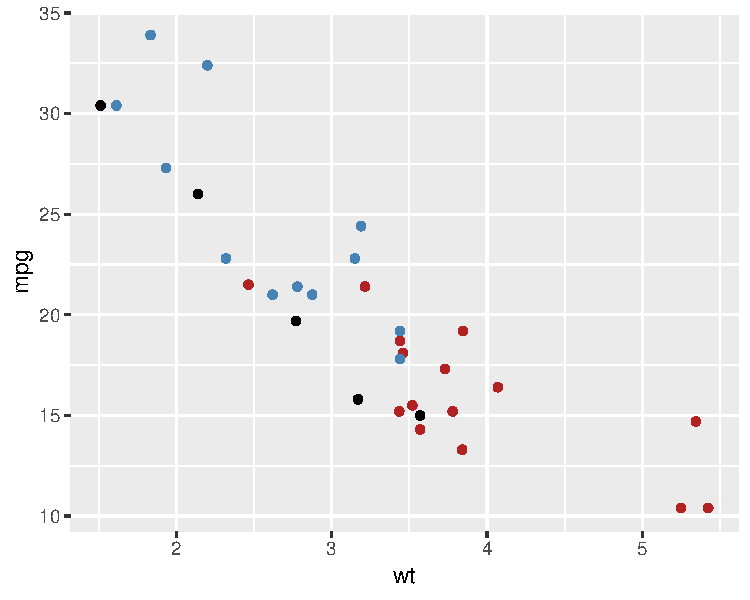
\includegraphics[width=0.7\linewidth]{ggplots2loon_files/figure-latex/multiple geom_points-1} \end{center}

To create the interactive plot, any of the \texttt{geom\_point} layers
could contribute to the active scatterplot model layer.

\begin{Shaded}
\begin{Highlighting}[]
\NormalTok{l_pgps.}\DecValTok{1}\NormalTok{ <-}\StringTok{ }\KeywordTok{loon.ggplot}\NormalTok{(pgps, }\DataTypeTok{linkingGroup =} \StringTok{"Motor Trend 1974"}\NormalTok{)}
\NormalTok{l_pgps.}\DecValTok{13}\NormalTok{ <-}\StringTok{ }\KeywordTok{loon.ggplot}\NormalTok{(pgps, }\DataTypeTok{activeGeomLayers =} \KeywordTok{c}\NormalTok{(}\DecValTok{1}\NormalTok{,}\DecValTok{3}\NormalTok{),}
                         \DataTypeTok{linkingGroup =} \StringTok{"Motor Trend 1974"}\NormalTok{)}
\NormalTok{l_pgps.}\DecValTok{123}\NormalTok{ <-}\StringTok{ }\KeywordTok{loon.ggplot}\NormalTok{(pgps, }\DataTypeTok{activeGeomLayers =} \KeywordTok{c}\NormalTok{(}\DecValTok{1}\NormalTok{, }\DecValTok{2}\NormalTok{, }\DecValTok{3}\NormalTok{),}
                         \DataTypeTok{linkingGroup =} \StringTok{"Motor Trend 1974"}\NormalTok{)}
\end{Highlighting}
\end{Shaded}

These plots now have different subsets of the points as their
scatterplot ``model'' or active layer.

\textbf{WARNING} The linking works as expected \emph{between these
three} plots but \textbf{not} with any of the other plots in the same
linking group. With a little extra care/work, this too is possible.

\subsubsection{\texorpdfstring{Forcing the correct linking --
\texttt{linkingKey}}{Forcing the correct linking -- linkingKey}}\label{forcing-the-correct-linking-linkingkey}

One solution to getting the linking correct is to force the
\texttt{linkingKey} of any new plot to match the keys already defined by
the other plots in the linking group.

The linking key of a loon plot is simply a character vector (default
here)

\begin{Shaded}
\begin{Highlighting}[]
\CommentTok{# this group's linking keys can be found from l_p1}
\NormalTok{groupKeys <-}\StringTok{ }\NormalTok{l_p1[}\StringTok{"linkingKey"}\NormalTok{]}
\NormalTok{groupKeys}
\CommentTok{#>  [1] "0"  "1"  "2"  "3"  "4"  "5"  "6"  "7"  "8"  "9"  "10" "11" "12" "13"}
\CommentTok{#> [15] "14" "15" "16" "17" "18" "19" "20" "21" "22" "23" "24" "25" "26" "27"}
\CommentTok{#> [29] "28" "29" "30" "31"}
\end{Highlighting}
\end{Shaded}

These values need to be selected and matched to the subsetting used by
the \texttt{geom\_point()} calls in the ggplot.

\begin{Shaded}
\begin{Highlighting}[]
\CommentTok{# the subsets were defined as}
\NormalTok{dataGeom1 <-}\StringTok{ }\NormalTok{mtcars}\OperatorTok{$}\NormalTok{gear }\OperatorTok{==}\StringTok{ }\DecValTok{3}
\NormalTok{dataGeom2 <-}\StringTok{ }\NormalTok{mtcars}\OperatorTok{$}\NormalTok{gear }\OperatorTok{==}\StringTok{ }\DecValTok{4}
\NormalTok{dataGeom3 <-}\StringTok{ }\NormalTok{mtcars}\OperatorTok{$}\NormalTok{gear }\OperatorTok{==}\StringTok{ }\DecValTok{5}
\end{Highlighting}
\end{Shaded}

As with \texttt{linkingGroup}, any change to \texttt{linkingKey} must
also declare whether the existing linked states are to be pushed to, or
pulled from, the group. Hence \texttt{l\_configure()} must be used.

\begin{Shaded}
\begin{Highlighting}[]
\KeywordTok{l_configure}\NormalTok{(l_pgps.}\DecValTok{1}\NormalTok{, }
            \DataTypeTok{linkingKey =}\NormalTok{ groupKeys[dataGeom1], }
            \DataTypeTok{sync =} \StringTok{"pull"}\NormalTok{)}
\KeywordTok{l_configure}\NormalTok{(l_pgps.}\DecValTok{13}\NormalTok{, }
            \DataTypeTok{linkingKey =} \KeywordTok{c}\NormalTok{(groupKeys[dataGeom1],}
\NormalTok{                           groupKeys[dataGeom3]), }
            \DataTypeTok{sync =} \StringTok{"pull"}\NormalTok{)}
\KeywordTok{l_configure}\NormalTok{(l_pgps.}\DecValTok{123}\NormalTok{, }
            \DataTypeTok{linkingKey =} \KeywordTok{c}\NormalTok{(groupKeys[dataGeom1],}
\NormalTok{                           groupKeys[dataGeom2],}
\NormalTok{                           groupKeys[dataGeom3]), }
            \DataTypeTok{sync =} \StringTok{"pull"}\NormalTok{)}
\end{Highlighting}
\end{Shaded}

\textbf{Alternatively}, the linking keys could be set up correctly when
the loon plot was created

\begin{Shaded}
\begin{Highlighting}[]
\NormalTok{l_pgps.}\DecValTok{23}\NormalTok{ <-}\StringTok{ }\KeywordTok{loon.ggplot}\NormalTok{(pgps, }
                         \DataTypeTok{linkingGroup =} \StringTok{"Motor Trend 1974"}\NormalTok{,}
                         \DataTypeTok{activeGeomLayers =} \KeywordTok{c}\NormalTok{(}\DecValTok{2}\NormalTok{,}\DecValTok{3}\NormalTok{),}
                         \DataTypeTok{linkingKey =} \KeywordTok{c}\NormalTok{(groupKeys[dataGeom2],}
\NormalTok{                                        groupKeys[dataGeom3])}
\NormalTok{                         )}
\end{Highlighting}
\end{Shaded}

\section{\texorpdfstring{Facets and \texttt{l\_compound}
plots}{Facets and l\_compound plots}}\label{facets-and-l_compound-plots}

A significant data analytic feature in the ggplot pipeline is the notion
of facetting the plots, for example, via \texttt{facet\_wrap()}

\begin{Shaded}
\begin{Highlighting}[]
\NormalTok{fwrap <-}\StringTok{ }\KeywordTok{ggplot}\NormalTok{(mtcars, }\KeywordTok{aes}\NormalTok{(}\DataTypeTok{x =}\NormalTok{ wt, }\DataTypeTok{y =}\NormalTok{ mpg)) }\OperatorTok{+}
\StringTok{  }\KeywordTok{geom_point}\NormalTok{() }\OperatorTok{+}
\StringTok{  }\KeywordTok{facet_wrap}\NormalTok{(}\OperatorTok{~}\StringTok{ }\NormalTok{gear }\OperatorTok{+}\StringTok{ }\NormalTok{am) }
\NormalTok{fwrap}
\end{Highlighting}
\end{Shaded}

\begin{center}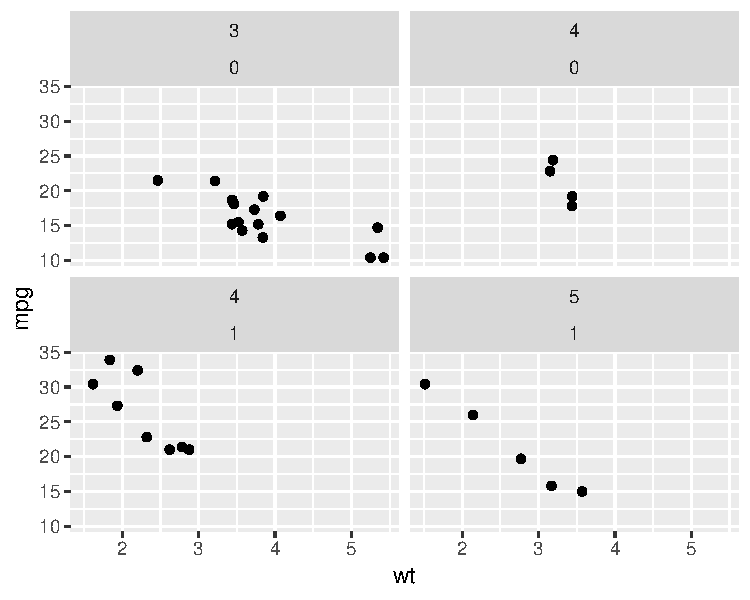
\includegraphics[width=0.7\linewidth]{ggplots2loon_files/figure-latex/fwrap-1} \end{center}

Facetted plots can also be rendered interactive in the same way as any
other ggplot:

\begin{Shaded}
\begin{Highlighting}[]
\NormalTok{l_fwrap <-}\StringTok{ }\KeywordTok{loon.ggplot}\NormalTok{(fwrap, }\DataTypeTok{linkingGroup =} \StringTok{"Motor Trend 1974"}\NormalTok{)}
\end{Highlighting}
\end{Shaded}

which will look like

\begin{center}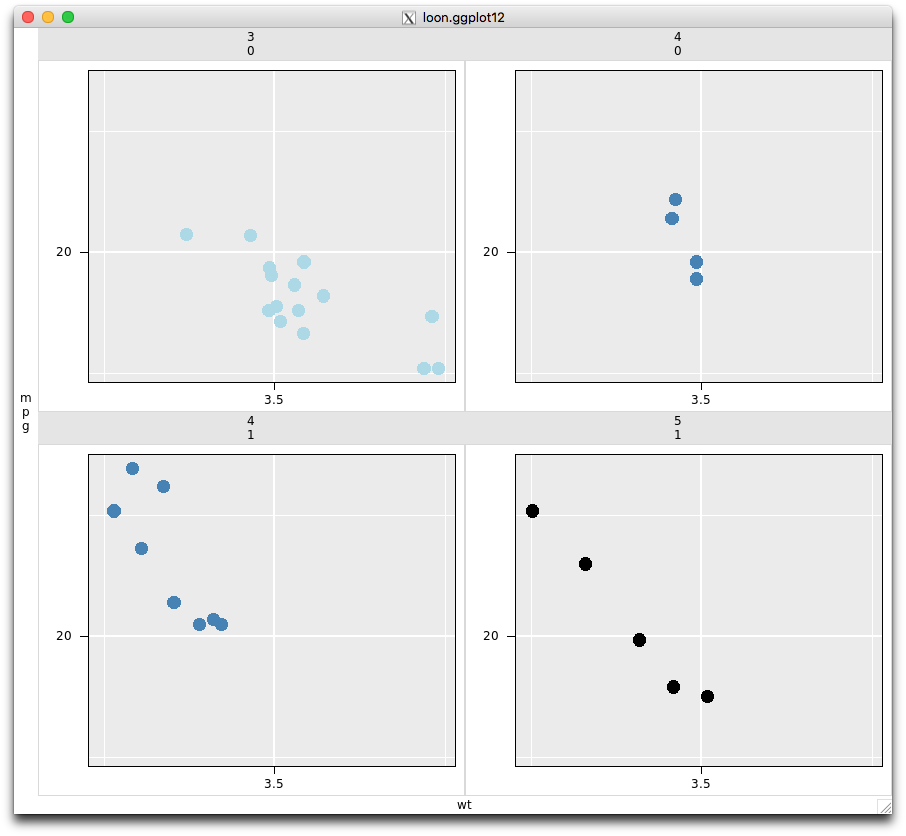
\includegraphics[width=0.7\linewidth]{./img/ggplots2loon//l_fwrap} \end{center}

Note that because we set the \texttt{linkingGroup} at the time of
creation (and because the \texttt{linkingKey} is the the default in all
plots in this group), the interactive facetted plot has pulled the
colours from the other plots in the same \texttt{linkingGroup}.

Note the class of \texttt{l\_fwrap}:

\begin{Shaded}
\begin{Highlighting}[]
\KeywordTok{class}\NormalTok{(l_fwrap)}
\CommentTok{#> [1] "l_ggplot"   "l_compound" "loon"}
\end{Highlighting}
\end{Shaded}

is an \texttt{l\_ggplot} because it is a loon rendition of a more
complex \texttt{ggplot},and it is an \texttt{l\_compound} which
indicates that it is a composition of individual loon plots.

As an \texttt{l\_compound} plot, other features of the composition can
be extracted. Such as the list of plots involved in the construction:

\begin{Shaded}
\begin{Highlighting}[]
\KeywordTok{l_getPlots}\NormalTok{(l_fwrap)}
\CommentTok{#> $x1y1}
\CommentTok{#> [1] ".12.plot"}
\CommentTok{#> attr(,"class")}
\CommentTok{#> [1] "l_plot" "loon"  }
\CommentTok{#> }
\CommentTok{#> $x1y2}
\CommentTok{#> [1] ".12.plot1"}
\CommentTok{#> attr(,"class")}
\CommentTok{#> [1] "l_plot" "loon"  }
\CommentTok{#> }
\CommentTok{#> $x2y1}
\CommentTok{#> [1] ".12.plot2"}
\CommentTok{#> attr(,"class")}
\CommentTok{#> [1] "l_plot" "loon"  }
\CommentTok{#> }
\CommentTok{#> $x2y2}
\CommentTok{#> [1] ".12.plot3"}
\CommentTok{#> attr(,"class")}
\CommentTok{#> [1] "l_plot" "loon"}
\end{Highlighting}
\end{Shaded}

as well as their layout in the composition

\begin{Shaded}
\begin{Highlighting}[]
\KeywordTok{l_getLocations}\NormalTok{(l_fwrap)}
\CommentTok{#>      [,1] [,2]}
\CommentTok{#> [1,]    1    2}
\CommentTok{#> [2,]    3    4}
\end{Highlighting}
\end{Shaded}

expressed as a matrix of the location of the plots in the order in which
they appear in \texttt{getPlots()}.

Each plot in \texttt{l\_fwrap} is an independent loon plot which can be
interacted with either through the inspector or programmatically.

\section{Pipes}\label{pipes}

THe \texttt{magrittr} package provides several different types of pipes
which can be a handy way to organize computation, especially when the
computation involves processing data for input to another procedure, in
this case \texttt{ggplot()}:

\begin{Shaded}
\begin{Highlighting}[]
\KeywordTok{library}\NormalTok{(tidyverse)  }\CommentTok{# load this to also have dplyr functionality}
\NormalTok{p1_piped <-}\StringTok{ }\NormalTok{mtcars }\OperatorTok
\StringTok{  }\KeywordTok{rename}\NormalTok{(}\DataTypeTok{transmission =}\NormalTok{ am, }\DataTypeTok{weight =}\NormalTok{ wt) }\OperatorTok
\StringTok{  }\KeywordTok{mutate}\NormalTok{(}\DataTypeTok{lp100km =}\NormalTok{ (}\DecValTok{100} \OperatorTok{*}\StringTok{ }\FloatTok{3.785411784}\NormalTok{) }\OperatorTok{/}\StringTok{ }\NormalTok{(}\FloatTok{1.609344} \OperatorTok{*}\StringTok{ }\NormalTok{mpg)) }\OperatorTok
\StringTok{  }\KeywordTok{select}\NormalTok{(weight, lp100km) }\OperatorTok
\StringTok{  }\KeywordTok{ggplot}\NormalTok{(}\KeywordTok{aes}\NormalTok{(}\DataTypeTok{x =}\NormalTok{ weight, }\DataTypeTok{y =}\NormalTok{ lp100km)) }\OperatorTok{+}
\StringTok{  }\KeywordTok{geom_point}\NormalTok{() }\OperatorTok{+}
\StringTok{  }\KeywordTok{ylab}\NormalTok{(}\StringTok{"Litres per 100 kilometres"}\NormalTok{) }\OperatorTok{+}
\StringTok{  }\KeywordTok{ggtitle}\NormalTok{(}\StringTok{"Gas usage"}\NormalTok{)}
\end{Highlighting}
\end{Shaded}

Here the ``pipe'' \texttt{\%\textgreater{}\%} takes the output of its
left hand side and pushes it into the first argument of its right hand
side. Arbitrary many pipes may be gathered together.\\
This connects nicely with \texttt{ggplot2}'s addition \texttt{+}
operator (\texttt{+} itself is sometimes a pipe, sometimes a layer in
\texttt{ggplot} construction) to create the \texttt{ggplot} from the
data and assign it to \texttt{p1\_piped}.

Two things to note here are. First, the result of the data manipulation
is assigned at the beginning using the \texttt{\textless{}-} assignment
function which seems to run counter to the data flow indicated by the
pipes. A more consistent flow would be to have instead written

\begin{Shaded}
\begin{Highlighting}[]
\NormalTok{mtcars }\OperatorTok
\StringTok{  }\KeywordTok{rename}\NormalTok{(}\DataTypeTok{transmission =}\NormalTok{ am, }\DataTypeTok{weight =}\NormalTok{ wt) }\OperatorTok
\StringTok{  }\KeywordTok{mutate}\NormalTok{(}\DataTypeTok{lp100km =}\NormalTok{ (}\DecValTok{100} \OperatorTok{*}\StringTok{ }\FloatTok{3.785411784}\NormalTok{) }\OperatorTok{/}\StringTok{ }\NormalTok{(}\FloatTok{1.609344} \OperatorTok{*}\StringTok{ }\NormalTok{mpg)) }\OperatorTok
\StringTok{  }\KeywordTok{select}\NormalTok{(weight, lp100km) }\OperatorTok
\StringTok{  }\KeywordTok{ggplot}\NormalTok{(}\KeywordTok{aes}\NormalTok{(}\DataTypeTok{x =}\NormalTok{ weight, }\DataTypeTok{y =}\NormalTok{ lp100km)) }\OperatorTok{+}
\StringTok{  }\CommentTok{#geom_point() +}
\StringTok{  }\KeywordTok{ylab}\NormalTok{(}\StringTok{"Litres per 100 kilometres"}\NormalTok{) }\OperatorTok{+}
\StringTok{  }\KeywordTok{ggtitle}\NormalTok{(}\StringTok{"Gas usage"}\NormalTok{)  ->}\StringTok{   }\CommentTok{# Note assignment occurs here}
\StringTok{  }\NormalTok{p1_piped}
\end{Highlighting}
\end{Shaded}

Now the assignment operator \texttt{-\textgreater{}} is used at the end,
matching the data flow of the pipes.

Second, in either case the \texttt{ggplot} is \textbf{not} itself
displayed (or rendered) until it is printed.

\begin{Shaded}
\begin{Highlighting}[]
\NormalTok{p1_piped}
\end{Highlighting}
\end{Shaded}

\begin{center}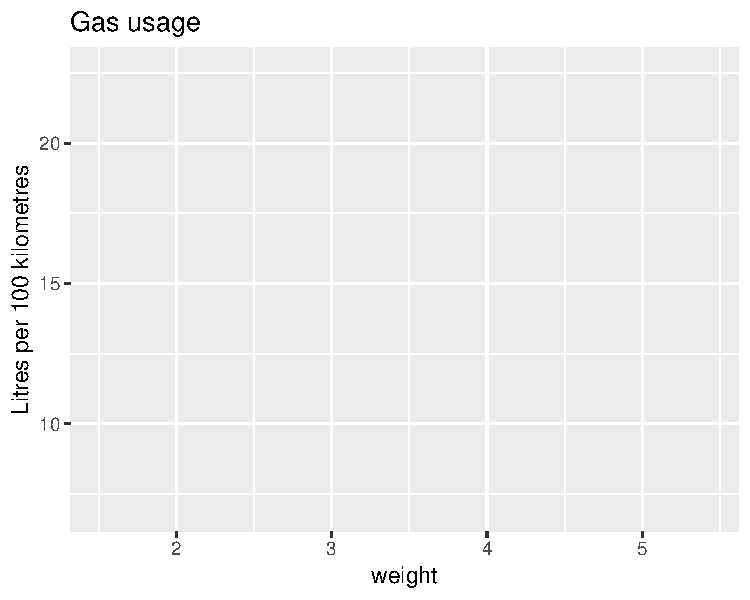
\includegraphics[width=0.7\linewidth]{ggplots2loon_files/figure-latex/p1_piped-1} \end{center}

Once built, as happens when the plot has been displayed as above, an
interactive loon plot can be had as always, simply by calling
\texttt{loon.ggplot()} on the built \texttt{ggplot}:

\begin{Shaded}
\begin{Highlighting}[]
\KeywordTok{loon.ggplot}\NormalTok{(p1_piped, }\DataTypeTok{linkingGroup =} \StringTok{"Motor Trend 1974"}\NormalTok{)}
\end{Highlighting}
\end{Shaded}

Again, the additional specification here of the \texttt{linkingGroup}
will cause display attributes to be pulled from the plots in that
linking group.

\subsection{\texorpdfstring{\texttt{gg\_pipe(data,\ ggplotObj)}}{gg\_pipe(data, ggplotObj)}}\label{gg_pipedata-ggplotobj}

Note that before a \texttt{ggplot} can be displayed, a number of steps
are performed so as to prepare the plot object for rendering (e.g.~see
\texttt{ggplot2::ggplot\_build}). Unfortunately, this delay in
completing the preparation of the \texttt{ggplot} can make it difficult
to attach further operations in the \texttt{\%\textgreater{}\%} pipeline
after the \texttt{ggplot} itself -- apart of course from further
\texttt{ggplot2} additions via the \texttt{+} operator. For example, one
cannot simply add \texttt{\%\textgreater{}\%\ loon.ggplot()} at the end
of the pipeline used to construct the \texttt{ggplot}. That is,

\begin{Shaded}
\begin{Highlighting}[]
\NormalTok{mtcars }\OperatorTok
\StringTok{  }\KeywordTok{rename}\NormalTok{(}\DataTypeTok{transmission =}\NormalTok{ am, }\DataTypeTok{weight =}\NormalTok{ wt) }\OperatorTok
\StringTok{  }\KeywordTok{mutate}\NormalTok{(}\DataTypeTok{lp100km =}\NormalTok{ (}\DecValTok{100} \OperatorTok{*}\StringTok{ }\FloatTok{3.785411784}\NormalTok{) }\OperatorTok{/}\StringTok{ }\NormalTok{(}\FloatTok{1.609344} \OperatorTok{*}\StringTok{ }\NormalTok{mpg)) }\OperatorTok
\StringTok{  }\KeywordTok{select}\NormalTok{(weight, lp100km) }\OperatorTok
\StringTok{  }\KeywordTok{ggplot}\NormalTok{(}\KeywordTok{aes}\NormalTok{(}\DataTypeTok{x =}\NormalTok{ weight, }\DataTypeTok{y =}\NormalTok{ lp100km)) }\OperatorTok{+}
\StringTok{  }\KeywordTok{geom_point}\NormalTok{() }\OperatorTok{+}
\StringTok{  }\KeywordTok{ylab}\NormalTok{(}\StringTok{"Litres per 100 kilometres"}\NormalTok{) }\OperatorTok{+}
\StringTok{  }\KeywordTok{ggtitle}\NormalTok{(}\StringTok{"Gas usage"}\NormalTok{) }\OperatorTok\StringTok{ }
\StringTok{  }\KeywordTok{loon.ggplot}\NormalTok{()}
\end{Highlighting}
\end{Shaded}

would produce neither a \texttt{ggplot} or an interactive \texttt{loon}
plot.

To get around this problem, in the \texttt{loon.ggplot} the function
\texttt{gg\_pipe()} is provided to encapsulate the \texttt{ggplot}
construction in any pipeline and force the \texttt{ggplot} to be built
(though not rendered in a display). The output of this function can then
be passed on to \texttt{loon.ggplot()}.

For example,

\begin{Shaded}
\begin{Highlighting}[]
\NormalTok{mtcars }\OperatorTok
\StringTok{  }\KeywordTok{rename}\NormalTok{(}\DataTypeTok{transmission =}\NormalTok{ am, }\DataTypeTok{weight =}\NormalTok{ wt) }\OperatorTok
\StringTok{  }\KeywordTok{mutate}\NormalTok{(}\DataTypeTok{lp100km =}\NormalTok{ (}\DecValTok{100} \OperatorTok{*}\StringTok{ }\FloatTok{3.785411784}\NormalTok{) }\OperatorTok{/}\StringTok{ }\NormalTok{(}\FloatTok{1.609344} \OperatorTok{*}\StringTok{ }\NormalTok{mpg)) }\OperatorTok
\StringTok{  }\KeywordTok{select}\NormalTok{(weight, lp100km) }\OperatorTok
\StringTok{  }\CommentTok{# encapsulate the ggplot construction with gg_pipe()}
\StringTok{  }\KeywordTok{gg_pipe}\NormalTok{(}\KeywordTok{ggplot}\NormalTok{(}\KeywordTok{aes}\NormalTok{(}\DataTypeTok{x =}\NormalTok{ weight, }\DataTypeTok{y =}\NormalTok{ lp100km)) }\OperatorTok{+}
\StringTok{            }\KeywordTok{geom_point}\NormalTok{() }\OperatorTok{+}
\StringTok{            }\KeywordTok{ylab}\NormalTok{(}\StringTok{"Litres per 100 kilometres"}\NormalTok{) }\OperatorTok{+}
\StringTok{            }\KeywordTok{ggtitle}\NormalTok{(}\StringTok{"Gas usage"}\NormalTok{)}
\NormalTok{          )  }\OperatorTok\StringTok{ }
\StringTok{  }\CommentTok{# and pass the built plot on}
\StringTok{  }\KeywordTok{loon.ggplot}\NormalTok{(}\DataTypeTok{linkingGroup =} \StringTok{"Motor Trend 1974"}\NormalTok{)}
\end{Highlighting}
\end{Shaded}

constructs the interactive plot which could have been assigned to a
variable as was done with the original \texttt{ggplot} construction.

From here, the pipeline can be grown as before, recognizing of course
that the output of \texttt{loon.ggplot()} is a \texttt{loon} plot of
some sort. This means that functions that operate on \texttt{loon} plots
(as their first argument can be used. As with any piping operation,
attention must be given to the first argument of the functions in the
pipeline as well as to what the input and outputs are of any function.

For example,

\begin{Shaded}
\begin{Highlighting}[]
\KeywordTok{library}\NormalTok{(magrittr)}
\NormalTok{mtcars }\OperatorTok
\StringTok{  }\KeywordTok{rename}\NormalTok{(}\DataTypeTok{transmission =}\NormalTok{ am, }\DataTypeTok{weight =}\NormalTok{ wt) }\OperatorTok
\StringTok{  }\KeywordTok{mutate}\NormalTok{(}\DataTypeTok{lp100km =}\NormalTok{ (}\DecValTok{100} \OperatorTok{*}\StringTok{ }\FloatTok{3.785411784}\NormalTok{) }\OperatorTok{/}\StringTok{ }\NormalTok{(}\FloatTok{1.609344} \OperatorTok{*}\StringTok{ }\NormalTok{mpg)) }\OperatorTok
\StringTok{  }\KeywordTok{select}\NormalTok{(weight, lp100km) }\OperatorTok
\StringTok{  }\CommentTok{# encapsulate the ggplot construction with gg_pipe()}
\StringTok{  }\KeywordTok{gg_pipe}\NormalTok{(}\KeywordTok{ggplot}\NormalTok{(}\KeywordTok{aes}\NormalTok{(}\DataTypeTok{x =}\NormalTok{ weight, }\DataTypeTok{y =}\NormalTok{ lp100km)) }\OperatorTok{+}
\StringTok{            }\KeywordTok{geom_point}\NormalTok{() }\OperatorTok{+}
\StringTok{            }\KeywordTok{ylab}\NormalTok{(}\StringTok{"Litres per 100 kilometres"}\NormalTok{) }\OperatorTok{+}
\StringTok{            }\KeywordTok{ggtitle}\NormalTok{(}\StringTok{"Gas usage"}\NormalTok{)}
\NormalTok{          )  }\OperatorTok\StringTok{ }
\StringTok{  }\CommentTok{# and pass the built plot on}
\StringTok{  }\KeywordTok{loon.ggplot}\NormalTok{(}\DataTypeTok{linkingGroup =} \StringTok{"Motor Trend 1974"}\NormalTok{) }\OperatorTok\StringTok{  }\CommentTok{# pipe the loon plot on}
\StringTok{  }\KeywordTok{l_cget}\NormalTok{(}\StringTok{'color'}\NormalTok{)  }\CommentTok{# Gets and returns the vector of point colours}
\CommentTok{#>  [1] "#46468282B4B4" "#46468282B4B4" "#46468282B4B4" "#ADADD8D8E6E6"}
\CommentTok{#>  [5] "#ADADD8D8E6E6" "#ADADD8D8E6E6" "#ADADD8D8E6E6" "#46468282B4B4"}
\CommentTok{#>  [9] "#46468282B4B4" "#46468282B4B4" "#46468282B4B4" "#ADADD8D8E6E6"}
\CommentTok{#> [13] "#ADADD8D8E6E6" "#ADADD8D8E6E6" "#ADADD8D8E6E6" "#ADADD8D8E6E6"}
\CommentTok{#> [17] "#ADADD8D8E6E6" "#46468282B4B4" "#46468282B4B4" "#46468282B4B4"}
\CommentTok{#> [21] "#ADADD8D8E6E6" "#ADADD8D8E6E6" "#ADADD8D8E6E6" "#ADADD8D8E6E6"}
\CommentTok{#> [25] "#ADADD8D8E6E6" "#46468282B4B4" "#000000000000" "#000000000000"}
\CommentTok{#> [29] "#000000000000" "#000000000000" "#000000000000" "#46468282B4B4"}
\end{Highlighting}
\end{Shaded}

In the \texttt{magrittr} package (the source of the pipeline operation)
there are a variety of pipeline operators which might also be useful --
not just \texttt{\%\textgreater{}\%}.

\subsection{just use loon for built-in interactive
plots}\label{just-use-loon-for-built-in-interactive-plots}

Of course, for plots already existing in \texttt{loon},
\texttt{ggplot()} and hence \texttt{gg\_pipe()} could be avoided
entirely:

\begin{Shaded}
\begin{Highlighting}[]
\NormalTok{mtcars }\OperatorTok
\StringTok{  }\KeywordTok{rename}\NormalTok{(}\DataTypeTok{transmission =}\NormalTok{ am, }\DataTypeTok{weight =}\NormalTok{ wt) }\OperatorTok
\StringTok{  }\KeywordTok{mutate}\NormalTok{(}\DataTypeTok{lp100km =}\NormalTok{ (}\DecValTok{100} \OperatorTok{*}\StringTok{ }\FloatTok{3.785411784}\NormalTok{) }\OperatorTok{/}\StringTok{ }\NormalTok{(}\FloatTok{1.609344} \OperatorTok{*}\StringTok{ }\NormalTok{mpg)) }\OperatorTok
\StringTok{  }\KeywordTok{select}\NormalTok{(weight, lp100km) }\OperatorTok
\StringTok{  }\CommentTok{# and pass the built plot on}
\StringTok{  }\KeywordTok{l_plot}\NormalTok{(}\DataTypeTok{title =} \StringTok{"Gas Usage"}\NormalTok{, }
         \DataTypeTok{showGuides =} \OtherTok{TRUE}\NormalTok{, }\DataTypeTok{showScales =} \OtherTok{TRUE}\NormalTok{,}
         \DataTypeTok{ylabel =} \StringTok{"Litres per 100 kilometres"}\NormalTok{, }
         \DataTypeTok{linkingGroup =} \StringTok{"Motor Trend 1974"}\NormalTok{) }\OperatorTok
\StringTok{  }\KeywordTok{grid.loon}\NormalTok{()   }\CommentTok{# get a static version via grid}
\end{Highlighting}
\end{Shaded}

\begin{center}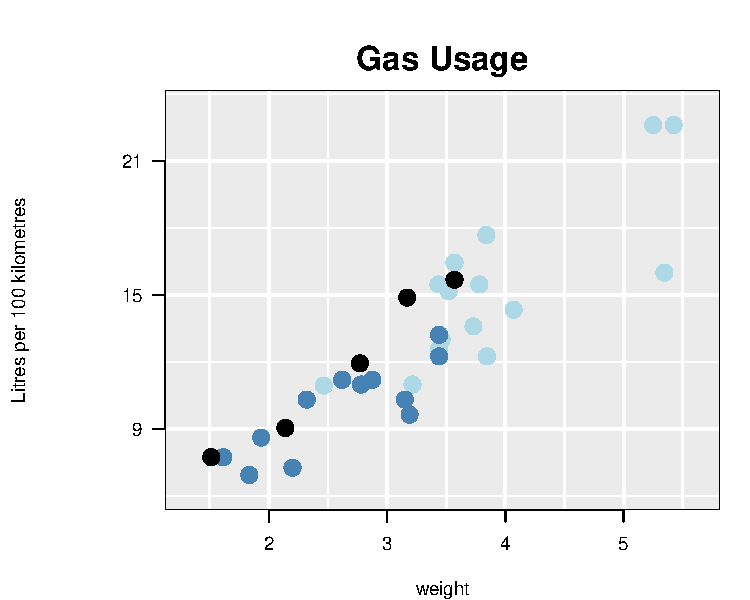
\includegraphics[width=0.7\linewidth]{ggplots2loon_files/figure-latex/loon only pipe-1} \end{center}

or

\begin{Shaded}
\begin{Highlighting}[]
\NormalTok{mtcars }\OperatorTok
\StringTok{  }\KeywordTok{rename}\NormalTok{(}\DataTypeTok{transmission =}\NormalTok{ am, }\DataTypeTok{weight =}\NormalTok{ wt) }\OperatorTok
\StringTok{  }\KeywordTok{mutate}\NormalTok{(}\DataTypeTok{lp100km =}\NormalTok{ (}\DecValTok{100} \OperatorTok{*}\StringTok{ }\FloatTok{3.785411784}\NormalTok{) }\OperatorTok{/}\StringTok{ }\NormalTok{(}\FloatTok{1.609344} \OperatorTok{*}\StringTok{ }\NormalTok{mpg)) }\OperatorTok
\StringTok{  }\KeywordTok{select}\NormalTok{(lp100km, weight, transmission) }\OperatorTok
\StringTok{  }\CommentTok{# and pass the built plot on}
\StringTok{  }\KeywordTok{l_pairs}\NormalTok{(}\DataTypeTok{showHistograms =} \OtherTok{TRUE}\NormalTok{,}
          \DataTypeTok{linkingGroup =} \StringTok{"Motor Trend 1974"}\NormalTok{) ->}\StringTok{  }\CommentTok{# and assign the result.}
\StringTok{  }\NormalTok{l_pp}
\end{Highlighting}
\end{Shaded}

produces an interactive pairs plot with histograms on the margins (see
\texttt{?l\_pairs}) and assigns the result to \texttt{l\_pp} (which
could have been assigned at the beginning with \texttt{\textless{}-} as
well).

\section{Other plots}\label{other-plots}


\end{document}
